% Options for packages loaded elsewhere
\PassOptionsToPackage{unicode}{hyperref}
\PassOptionsToPackage{hyphens}{url}
%
\documentclass[
]{article}
\usepackage{amsmath,amssymb}
\usepackage{iftex}
\ifPDFTeX
  \usepackage[T1]{fontenc}
  \usepackage[utf8]{inputenc}
  \usepackage{textcomp} % provide euro and other symbols
\else % if luatex or xetex
  \usepackage{unicode-math} % this also loads fontspec
  \defaultfontfeatures{Scale=MatchLowercase}
  \defaultfontfeatures[\rmfamily]{Ligatures=TeX,Scale=1}
\fi
\usepackage{lmodern}
\ifPDFTeX\else
  % xetex/luatex font selection
\fi
% Use upquote if available, for straight quotes in verbatim environments
\IfFileExists{upquote.sty}{\usepackage{upquote}}{}
\IfFileExists{microtype.sty}{% use microtype if available
  \usepackage[]{microtype}
  \UseMicrotypeSet[protrusion]{basicmath} % disable protrusion for tt fonts
}{}
\makeatletter
\@ifundefined{KOMAClassName}{% if non-KOMA class
  \IfFileExists{parskip.sty}{%
    \usepackage{parskip}
  }{% else
    \setlength{\parindent}{0pt}
    \setlength{\parskip}{6pt plus 2pt minus 1pt}}
}{% if KOMA class
  \KOMAoptions{parskip=half}}
\makeatother
\usepackage{xcolor}
\usepackage[margin=1in]{geometry}
\usepackage{longtable,booktabs,array}
\usepackage{calc} % for calculating minipage widths
% Correct order of tables after \paragraph or \subparagraph
\usepackage{etoolbox}
\makeatletter
\patchcmd\longtable{\par}{\if@noskipsec\mbox{}\fi\par}{}{}
\makeatother
% Allow footnotes in longtable head/foot
\IfFileExists{footnotehyper.sty}{\usepackage{footnotehyper}}{\usepackage{footnote}}
\makesavenoteenv{longtable}
\usepackage{graphicx}
\makeatletter
\def\maxwidth{\ifdim\Gin@nat@width>\linewidth\linewidth\else\Gin@nat@width\fi}
\def\maxheight{\ifdim\Gin@nat@height>\textheight\textheight\else\Gin@nat@height\fi}
\makeatother
% Scale images if necessary, so that they will not overflow the page
% margins by default, and it is still possible to overwrite the defaults
% using explicit options in \includegraphics[width, height, ...]{}
\setkeys{Gin}{width=\maxwidth,height=\maxheight,keepaspectratio}
% Set default figure placement to htbp
\makeatletter
\def\fps@figure{htbp}
\makeatother
\setlength{\emergencystretch}{3em} % prevent overfull lines
\providecommand{\tightlist}{%
  \setlength{\itemsep}{0pt}\setlength{\parskip}{0pt}}
\setcounter{secnumdepth}{5}
% definitions for citeproc citations
\NewDocumentCommand\citeproctext{}{}
\NewDocumentCommand\citeproc{mm}{%
  \begingroup\def\citeproctext{#2}\cite{#1}\endgroup}
\makeatletter
 % allow citations to break across lines
 \let\@cite@ofmt\@firstofone
 % avoid brackets around text for \cite:
 \def\@biblabel#1{}
 \def\@cite#1#2{{#1\if@tempswa , #2\fi}}
\makeatother
\newlength{\cslhangindent}
\setlength{\cslhangindent}{1.5em}
\newlength{\csllabelwidth}
\setlength{\csllabelwidth}{3em}
\newenvironment{CSLReferences}[2] % #1 hanging-indent, #2 entry-spacing
 {\begin{list}{}{%
  \setlength{\itemindent}{0pt}
  \setlength{\leftmargin}{0pt}
  \setlength{\parsep}{0pt}
  % turn on hanging indent if param 1 is 1
  \ifodd #1
   \setlength{\leftmargin}{\cslhangindent}
   \setlength{\itemindent}{-1\cslhangindent}
  \fi
  % set entry spacing
  \setlength{\itemsep}{#2\baselineskip}}}
 {\end{list}}
\usepackage{calc}
\newcommand{\CSLBlock}[1]{\hfill\break\parbox[t]{\linewidth}{\strut\ignorespaces#1\strut}}
\newcommand{\CSLLeftMargin}[1]{\parbox[t]{\csllabelwidth}{\strut#1\strut}}
\newcommand{\CSLRightInline}[1]{\parbox[t]{\linewidth - \csllabelwidth}{\strut#1\strut}}
\newcommand{\CSLIndent}[1]{\hspace{\cslhangindent}#1}
\usepackage{setspace}\linespread{1.25}
\usepackage[fontsize=12pt]{scrextend}
\usepackage[left]{lineno}
\usepackage[labelformat=empty]{caption}
\usepackage{longtable}
\usepackage{booktabs}
\ifLuaTeX
  \usepackage{selnolig}  % disable illegal ligatures
\fi
\usepackage{bookmark}
\IfFileExists{xurl.sty}{\usepackage{xurl}}{} % add URL line breaks if available
\urlstyle{same}
\hypersetup{
  hidelinks,
  pdfcreator={LaTeX via pandoc}}

\author{}
\date{\vspace{-2.5em}}

\begin{document}

\textbf{N-Methyl-D-aspartate receptor hypofunction causes recurrent and
transient failures of perceptual inference}\\
\strut \\

\textbf{Authors}:

Veith Weilnhammer\(^{1,2, 3,ec}\), Marcus Rothkirch\(^{1, 4, ec}\),
Deniz Yilmaz\(^{1,5,6,7, ec}\), Merve Fritsch\(^{1}\), Lena Esther
Ptasczynski\(^{1,5}\), Katrin Reichenbach\(^{1}\), Lukas
Rödiger\(^{1}\), Philip Corlett\(^{8}\), Philipp Sterzer\(^{9}\)\\
\strut \\
\textbf{Affiliations}:

\(^{1}\) Department of Psychiatry, Charité-Universitätsmedizin Berlin,
corporate member of Freie Universität Berlin and Humboldt-Universität zu
Berlin, Germany\\
\(^{2}\) Berlin Institute of Health, Charité-Universitätsmedizin Berlin
and Max Delbrück Center, Germany\\
\(^{3}\) Helen Wills Neuroscience Institute, University of California
Berkeley, USA\\
\(^{4}\) Medical School Berlin, Hochschule für Gesundheit und Medizin,
Germany\\
\(^{5}\) Berlin School of Mind and Brain, Humboldt-Universität zu
Berlin, Germany\\
\(^{6}\) Max Planck School of Cognition, Leipzig, Germany\\
\(^{7}\) Department of Psychiatry and Psychotherapy, LMU University
Hospital, Munich, Germany\\
\(^{8}\) Department of Psychiatry, Yale University School of Medicine,
New Haven, USA\\
\(^{9}\) Department of Psychiatry (UPK), University of Basel,
Switzerland\\
\strut \\
\textbf{Contributions}:

\(^{ec}\) Equal contribution\\
\strut \\
\textbf{Corresponding Author}:

Veith Weilnhammer, Helen Wills Neuroscience Institute, University of
California Berkeley, USA, email:
\href{mailto:veith.weilnhammer@gmail.com}{\nolinkurl{veith.weilnhammer@gmail.com}}\\

\textbf{Running Title}: Failures of inference under ketamine

\textbf{Keywords}: schizophrenia, psychosis, ketamine, predictive
processing, bistable perception, modes of inference

\newpage

\linenumbers

\section{Abstract}\label{abstract}

Perception integrates external sensory signals with internal predictions
that reflect prior knowledge about the world. Previous research suggests
that this integration is governed by slow alternations between an
external mode, driven by sensory signals, and an internal mode, shaped
by prior knowledge. Using a double-blind, placebo-controlled, cross-over
experiment in healthy human participants, we investigated the effects of
the N-Methyl-D-aspartate receptor (NMDAR) antagonist S-ketamine on the
balance between external and internal modes. We found that S-ketamine
causes a shift of perception toward the external mode. A case-control
study revealed that individuals with paranoid Scz, a disorder repeatedly
associated with NMDAR hypofunction, spend more time in the external
mode. This NMDAR-dependent increase in the external mode suggests that
the symptoms of schizophrenia are caused by recurring dissociations of
perception from prior knowledge about the world.

\section{Introduction}\label{introduction}

Imagine a dimly lit room at a crowded party, where unclear visual
signals, indistinct sounds, and complex social interactions allow for
multiple - and sometimes false - interpretations. In such ambiguity,
failures of perceptual inference, the ability to contextualize sensory
inputs with prior knowledge about the world, can lead to profound
departures from reality: Faces obscured in shadow may appear distorted,
random noise could be perceived as a whisper, and friendly smiles might
seem derogatory.

According to the canonical predictive processing
hypothesis\textsuperscript{1}, a disruption of perceptual inference is
likely to play a crucial role in schizophrenia (Scz), a severe mental
disorder characterized by psychotic symptoms such as delusions and
hallucinations\textsuperscript{1}. People with Scz may fail to apply
prior knowledge to the interpretation of ambiguous sensory signals,
causing erratic inferences that lead to hallucinatory experiences and
delusional beliefs\textsuperscript{1}. Yet despite considerable progress
in the computational understanding of psychosis, two key questions have
remained unanswered.

The first question concerns the neural mechanisms that cause perceptual
inference to fail in Scz. Formal predictive processing accounts of Scz
foreground the role of prediction errors in updating Bayesian beliefs
about the causes of sensory input\textsuperscript{2}. Most accounts
focus on a failure to predict or instantiate the precision afforded to
prediction errors at various levels of the cortical
hierarchy\textsuperscript{1}. Precision refers to the confidence
ascribed to prediction errors, and regulates how prior expectations are
updated in response to sensory information\textsuperscript{2}.
Mathematically, precision is equivalent to the (Kalman) gain or the
weighting of prediction errors in predictive processing models of
perceptual inference\textsuperscript{3}. Psychologically, the deployment
of sensory precision can be understood in terms of selective attention
(or sensory attenuation)\textsuperscript{4}. Physiologically, precision
corresponds to the postsynaptic gain or excitability of neuronal
populations that report prediction errors, commonly mediated by
N-Methyl-D-aspartate receptors\textsuperscript{5} (NMDARs).

Beyond predictive processing theory, several lines of evidence point to
NMDAR hypofunction as a key factor in the pathophysiology of
psychosis\textsuperscript{6}. NMDAR antibodies\textsuperscript{7} and
antagonists such as ketamine\textsuperscript{8} mimic the symptoms of
Scz, which is itself associated with a reduction of NMDAR density in the
prefrontal cortex\textsuperscript{9}. In addition to their role in
controlling the excitability of prediction error
neurons\textsuperscript{6} and their general function for maintaining
the cortical excitation-inhibition balance\textsuperscript{10}, NMDARs
play a critical role in cortical feedback\textsuperscript{11}, support
synaptic short-term plasticity\textsuperscript{12}, and interact with
neuromodulators such as dopamine and serotonin via GABAergic
interneurons\textsuperscript{13}. While these NMDAR-dependent mechanisms
are likely critical for perceptual inference, it is yet to be determined
how NMDAR hypofunction may cause the symptoms of Scz.

The second unresolved question concerns the temporal dynamics of
psychotic experiences, which often unfold as short-lived events spanning
from seconds to minutes, especially at early stages of Scz. The
transient nature of psychotic experiences challenges models that assume
a constant disruption of perceptual inference\textsuperscript{1}. A
solution to this problem is suggested by the recent observation that
perceptual inference is subject to spontaneous fluctuations over
time\textsuperscript{14}. Such fluctuations have been related to two
opposing modes of inference, or shifts in attentional sets, during which
perception is driven predominantly either by external inputs (external
mode) or by internal predictions that stem from recent
experiences\textsuperscript{15} (internal mode, Figure 1A). Although
preliminary evidence indicates a tendency toward the external mode in
people with Scz\textsuperscript{16}, the neural mechanisms of mode
fluctuations and their potential implications for computational models
of Scz have remained elusive.

The objective of the current study was therefore twofold: First, to test
whether NMDAR hypofunction causes changes in perceptual inference that
characterize Scz; and second, to explore the effect of NMDAR
hypofunction on ongoing fluctuations in perceptual inference that may
explain the transient nature of psychotic experiences. We addressed
these questions in a double-blind, placebo-controlled, cross-over
experiment with S-ketamine in healthy participants, and a case-control
study that compared patients with paranoid Scz to matched healthy
controls\textsuperscript{17}. Participants engaged in a task designed to
test how internal predictions derived from previous experiences modulate
the perception of sensory signals that varied in ambiguity. We found
that NMDAR antagonism and Scz were associated with a shift of perception
toward the external mode, a minute-long state of the brain during which
inference dissociates from prior knowledge. Our results suggest that
NMDAR hypofunction shifts the balance between external and internal
modes, and may thus contribute to the symptoms of Scz by causing
transient and recurring failures of perceptual inference.

\section{Materials and Methods}\label{materials-and-methods}

For details on the experimental paradigm, participant recruitment and
consent, inclusion/exclusion criteria, randomization and blinding, drug
administration protocols, safety monitoring, data analysis, and
computational modeling, please refer to Supplemental Methods S1.

\section{Results}\label{results}

To investigate whether NMDAR hypofunction influences perceptual
inference, and how NMDAR hypofunction contributes to the transient
nature of psychotic experiences, we conducted a double-blind
placebo-controlled cross-over experiment in 28 healthy human
participants. The participants attended two experimental sessions during
which they received a continuous intravenous infusion of either the
NMDAR antagonist S-ketamine at a dose of 0.1 mg/kg/h or a saline
placebo. In each session, the participants viewed ten 120 sec blocks of
an ambiguous structure-from-motion (SFM) stimulus that induced the
experience of a sphere rotating around a vertical axis, and reported
changes in the perceived direction of rotation (leftward vs.~rightward
movement of the front surface) as well as their confidence in the choice
(Figure 1B and Supplemental Video S1).

The ambiguity of the display induced the phenomenon of bistable
perception: Even though the stimulus was physically ambiguous at each
frame of the presentation, spontaneous changes in the perceived
direction of rotation occurred in average intervals of \(13.75\) ±
\(3.09\) sec.~In line with previous results\textsuperscript{17,18},
these changes in perception occurred with a probability of \(0.11\) ±
\(\ensuremath{8.67\times 10^{-3}}\) at brief depth-symmetric
configurations of the stimulus (see Supplemental Video S1 and
Supplemental Figure S2A). We therefore divided the continuous behavioral
reports into a sequence of discrete states t. Each state was associated
with a perceptual experience \(y_t\), confidence \(c_t\) and the
external input \(s_t\).

Predictive processing conceptualizes bistable perception as an
inferential process about the cause of \(s_t\). The core idea is that
previous experiences (\(y_{t-1}\)) generate internal predictions that
bias the interpretation \(y_t\) of the ambiguous
stimulus\textsuperscript{18} (Figure 1C). In this view, inferences
during bistability mirror the temporal autocorrelation of natural
environments, where the recent past typically predicts the near future,
much like frames captured by a video camera allow for the prediction of
future frames\textsuperscript{19}. The adaptive benefit of this
predictive strategy is the stabilization of perception that prevents
erratic experiences in natural environments, which are highly
autocorrelated and accessible to the brain only via inherently ambiguous
sensory signals\textsuperscript{2}.

Predictive processing models of bistable perception assume that
transitions between the alternative interpretations of (partially)
ambiguous stimuli are driven by conflicts between the external input and
stabilizing internal predictions\textsuperscript{17,18}. To test how
NMDAR antagonism alters the balance between external inputs and internal
predictions, we attached a 3D signal to a fraction of the stimulus dots.
The signal-to-ambiguity ratio (SAR) ranged from complete ambiguity to
full disambiguation across five levels and remained constant in each
block of the experiment. By changing the direction of rotation enforced
by the 3D signal at random in average intervals of 10 sec, we created
dynamic conflicts between the SAR-weighted input \(s_t\) and the
stabilizing internal prediction \(y_{t-1}\). Due to the random changes
in \(s_t\), a shift of inference away from internal predictions and
toward external sensory data, which has repeatedly been associated with
NMDAR hypofunction\textsuperscript{1} and may be maladaptive in
autocorrelated natural environments\textsuperscript{15}, should manifest
as an increase in perceptual accuracy in our experiment.

\subsection{NMADR hypofunction shifts perceptual inference toward the
external input and away from internal
predictions}\label{nmadr-hypofunction-shifts-perceptual-inference-toward-the-external-input-and-away-from-internal-predictions}

As expected, we found that \(y_t\) was driven by both \(s_t\) (\(\beta\)
= \(3.01\) ± \(0.06\), z = \(50.39\), p = \(0\)) and \(y_{t-1}\)
(\(\beta\) = \(2.06\) ± \(0.03\), z = \(80.58\), p = \(0\)).
Importantly, S-ketamine caused perception to shift toward \(s_t\)
(\(\beta\) = \(0.45\) ± \(0.08\), z = \(5.6\), p =
\(\ensuremath{1.71\times 10^{-7}}\), Figure 2A and Supplemental Figure
S3), indicating a stronger weighting of external inputs over internal
predictions during pharmacologically induced NMDAR hypofunction. Under
the predictive processing formulation of perceptual inference, one can
read the estimates for \(s_t\) and \(y_{t-1}\) as sensory and prior
precision, respectively. This suggests that S-ketamine augments sensory
precision by altering the interactions between pyramidal cells and
fast-spiking inhibitory interneurons thought to underwrite cortical gain
control or excitation-inhibition balance\textsuperscript{10}.

Next, we performed the same analysis on data from a previous
case-control study using an analogous task in patients with
Scz\textsuperscript{17}. In Scz patients and controls, \(y_t\) was
influenced by the SAR-weighted input \(s_t\) (\(\beta\) = \(2.77\) ±
\(0.11\), z = \(-24.85\), p = \(\ensuremath{2.18\times 10^{-135}}\)) and
the stabilizing prediction \(y_{t-1}\) (\(\beta\) = \(1.5\) ± \(0.03\),
z = \(-58.2\), p = \(0\)). Similar to S-ketamine, \(s_t\) had a larger
impact on perception in Scz patients than controls (\(\beta\) = \(0.75\)
± \(0.15\), z = \(4.96\), p = \(\ensuremath{5.6\times 10^{-6}}\), Figure
2E and Supplemental Figure S4).

Together, these results align with the canonical predictive processing
theory of Scz\textsuperscript{1}: Pharmacologically-induced NMDAR
hypofunction and Scz are associated with a shift of perceptual inference
toward external inputs, and away from stabilizing internal predictions.
This increase in sensory precision (relative to prior precision) is
often framed as a failure of sensory attenuation, i.e., the inability to
attenuate sensory precision or, psychologically, ignore unclear or
irrelevant sensations\textsuperscript{20}. In the artificial setting of
our experiment, where stimuli are random, weak internal predictions
under S-ketamine and in Scz lead to \emph{increased} perceptual
accuracy. In autocorrelated natural environments, however, NMDAR
hypofunction may trigger psychotic experiences by causing erratic
inferences about ambiguous sensory information.

\subsection{NMDAR-dependent changes of perceptual inference stem from an
altered balance between external and internal modes of
perception}\label{nmdar-dependent-changes-of-perceptual-inference-stem-from-an-altered-balance-between-external-and-internal-modes-of-perception}

As a mechanism for symptoms that are transient and recurring,
NMDAR-dependent changes in perceptual inference should not be constant,
but fluctuate dynamically at a timescale that is compatible with the
duration of individual psychotic experiences. We tested this prediction
in Hidden Markov Models (HMM) that inferred transitions between two
latent states, each linked to an independent general linear model (GLM)
that predicted \(y_t\) from \(s_t\) and \(y_{t-1}\). The \(\beta\)
weights quantified the sensitivity to ambiguous sensory information
(\(\beta_S \times s_t\)) relative to the stabilizing effect of internal
predictions provided by preceding experiences
(\(\beta_{P} \times y_{t-1}\)), and allowed us to evaluate dynamic
changes in the balance \(\Delta_{S-P} = \beta_S - \beta_P\) between the
two.

Consistent with recent findings in humans and
mice\textsuperscript{14,15}, Bayesian model comparison indicated a clear
superiority of the two-state GLM-HMM over the standard one-state GLM in
the S-ketamine experiment (\(\delta_{BIC}\) =
\(\ensuremath{-3.65\times 10^{3}}\)). According to the two-state
GLM-HMM, perception fluctuated between an internal mode, shaped by the
stabilizing internal prediction \(y_{t-1}\), and an external mode,
dominated by the SAR-weighted input \(s_t\). External mode increased
\(\Delta_{S-P}\) by \(2.8\) ± \(0.29\) (T(\(81\)) = \(9.5\), p =
\(\ensuremath{5.22\times 10^{-13}}\), Figure 2B-C). Switches between
modes occurred in intervals of \(179.97\) ± \(19.39\) sec.~

The presence of slow fluctuations between external and internal modes
suggests that, instead of causing a constant increase in the sensitivity
to external inputs, NMDAR hypofunction may affect perception by shifting
the dynamic balance between the two modes. Indeed, S-ketamine did not
alter the weights of the two-state GLM-HMM (Figure 2C), but increased
the probability of external at the expense of internal mode (\(\beta\) =
\(1.01\) ± \(0.03\), z = \(30.7\), p =
\(\ensuremath{4.26\times 10^{-206}}\), Figure 2D) via an effect on the
stay transitions of the HMM (external-to-external and
internal-to-internal, Supplemental Figure S3D). This effect was stable
over time, and present across the full range of SAR (Figure 2D).
Inter-individual differences in the effects of S-ketamine confirmed that
NMDAR hypofunction raised the sensitivity to sensory information (Figure
2A) by modulating the time participants spent in external and internal
modes, respectively (\(\rho\) = \(0.41\), T(\(26\)) = \(2.3\), p =
\(0.03\)). Our results therefore suggest that the failure of sensory
attenuation observed under S-ketamine corresponds to an inability to
disengage the external mode of perception. Through the lens of
predictive processing, the external mode reflects a state of perception
that is characterized by an increase in sensory precision at the expense
of prior precision. Crucially, it is this balance between sensory and
prior precision that determines the Kalman gain. In other words, what
matters in terms of perceptual inference are the dynamic changes in
relative precision over time.

Strikingly, the data from the Scz-control study mirrored the effect of
S-ketamine on the balance between external and internal mode: The
two-state GLM-HMM outperformed the standard one-state GLM (patients:
\(\delta_{BIC}\) = \(-981.65\); controls: \(\delta_{BIC}\) =
\(-862.91\)) and revealed two opposing modes (\(\Delta_{S-P}\) =
\(1.44\) ± \(0.33\), T(\(44\)) = \(4.33\), p =
\(\ensuremath{3.39\times 10^{-4}}\), Figure 2F) that alternated in
intervals of \(265.38\) ± \(57.76\) sec for patients and \(230.99\) ±
\(65.04\) sec for controls. Patients and controls did not differ with
respect to the weights of the two-state GLM-HMM (Figure 2G). Instead,
Scz patients spent more time in external mode (\(\beta\) = \(0.52\) ±
\(0.03\), z = \(16.88\), p = \(\ensuremath{1.23\times 10^{-63}}\),
Figure 2H and Supplemental Figure 4D).

\subsection{External and internal modes are perceptual phenomena that
cannot be reduced to fluctuations in arousal, fatigue, task engagement,
or task
difficulty}\label{external-and-internal-modes-are-perceptual-phenomena-that-cannot-be-reduced-to-fluctuations-in-arousal-fatigue-task-engagement-or-task-difficulty}

Our results suggest that healthy participants under S-ketamine and Scz
patients spend more time in the external mode. As a dynamic mechanism
for psychotic experiences, alternations between external and internal
mode should have an effect at the level of perception. This means that
between-mode alternations should modulate a perceptual decision variable
that determines not only what is consciously experienced, but also how
the contents of perception are evaluated by downstream cognition. The
hypothesis that external and internal modes are perceptual phenomena
needs to be contrasted against alternative scenarios in which external
and internal modes are driven primarily by fluctuations in arousal,
high-level cognition, or executive function. This is particularly
important, as behavioral reports served as the sole indicators of
perceptual states in our paradigm.

To address these alternative accounts, we first performed additional
tests to support our claim that external and internal mode operate at
the level of perception. External and internal modes are states of a
GLM-HMM that integrates the external stimulus \(s_t\) with the previous
experience \(y_{t-1}\) into a perceptual decision variable
\(P(y_t = 1)\). The parameters of the GLM-HMM are optimized to predict
the sequence of perceptual experiences \(y_t\) from \(P(y_t = 1)\). If
external and internal modes are perceptual phenomena, then the
stabilization of perception should be driven by the sequence of
experiences \(y_t\), as opposed to the sequence of stimuli \(s_t\). To
test this hypothesis, we compared our \emph{experienced-based} GLM-HMM,
in which the stabilizing internal predictions are driven by the
participants' perceptual experience at the preceding overlap, with an
alternative \emph{stimulus-based} GLM, in which the stabilizing internal
predictions are driven by the stimulus presented at the preceding
overlap. Bayesian model comparison indicated that the experienced-based
GLM-HMM was better at explaining our data than a stimulus-based GLM-HMM
in the S-ketamine experiment (\(\delta_{BIC}\) =
\(\ensuremath{-7.4\times 10^{3}}\)) and the case-control study
(patients: \(\delta_{BIC}\) = \(-981.65\); controls: \(\delta_{BIC}\) =
\(-862.91\)).

Moreover, if external and internal modes are perceptual phenomena, then
the decision variable \(P(y_t = 1)\) should not only determine the
contents of perception, but also metacognitive processes that depend on
them. To assess this prediction, we tested whether the posterior
certainty \(C_t\) at which the GLM-HMM predicted the content of
perception, i.e., the log probability of the experience \(y_t\) given
the decision variable \(P(y_t = 1)\)
(\(C_t = y_t \cdot \log(P(y_t = 1)) + (1 - y_t) \cdot \log(1 - P(y_t = 1))\)),
would correlate with the confidence reports \(c_t\) in the S-ketamine
experiment. This test is a powerful validation of our approach, since
the GLM-HMM was only fitted to binary perceptual states \(y_t\), and not
to the confidence \(c_t\) at which they were reported. Indeed, \(C_t\)
predicted the confidence reports \(c_t\) (\(\beta\) = \(0.29\) ±
\(0.02\), z = \(15.4\), p = \(\ensuremath{1.54\times 10^{-53}}\))
without an interaction with mode (\(\beta\) = \(-0.07\) ± \(0.07\), z =
\(-1.03\), p = \(0.3\)), confirming that the positive correlation
between posterior certainty and confidence was present in both external
and internal modes. \(C_t\) extracted from the two-state GLM-HMM was
better at explaining confidence than the one-state control GLM
(\(\delta_{BIC}\) = -280.69), and the one-state stimulus GLM
(\(\delta_{BIC}\) = -445.13).

As a consequence, internal mode should be associated with lower
metacognitive performance (i.e., the degree to which confidence
correlates accuracy), since stabilizing internal predictions have a
larger effect on perception in the internal mode, and cause experiences
\(y_t\) to be less constrained by the external input \(s_t\). Indeed,
accuracy was predictive of high confidence (\(\beta\) = \(1.01\) ±
\(0.05\), z = \(18.7\), p = \(\ensuremath{4.63\times 10^{-78}}\)), but
to a lesser degree during the internal mode (\(\beta\) = \(-0.61\) ±
\(0.09\), z = \(-6.61\), p = \(\ensuremath{3.94\times 10^{-11}}\)). In
line with this, metacognitive sensitivity, as measured by meta-d', was
significantly lower in the internal mode (\(\beta\) = \(-1.6\) ±
\(0.45\), T(\(50\)) = \(-3.55\), p =
\(\ensuremath{3.41\times 10^{-3}}\)). Together, these findings support
the hypothesis that external and internal modes modulate a low-level
decision variable \(P(y_t = 1)\) that determines the content of
perception and their metacognitive evaluation.

Second, we asked whether fluctuations in global brain states can provide
an alternative explanation for external and internal modes. One could
assume that mode alternations could in fact reflect dynamic states of
arousal, with high arousal and engaged behavior corresponding to the
external mode, and low arousal and disengaged behavior corresponding to
the internal mode. Our time-resolved assessment of internal states
revealed reduced wakefulness (Q1) under S-ketamine (Supplemental Figure
S6). This observation is clearly incompatible with the hypothesis that
changes in the dynamics of mode are driven by low arousal under
S-ketamine, since NMDAR antagonism increased the prevalence of the
external mode, improving behavioral performance in the artificial
setting of our experiment. When controlling for dynamic changes in
wakefulness (Q1), subjective intoxication (Q2) and nervousness (Q3), the
effect of S-ketamine on mode (p = \(\ensuremath{8.21\times 10^{-67}}\))
and the effect of mode on \(\Delta_{S-P}\) remained significant (p =
\(\ensuremath{1.29\times 10^{-5}}\)). We observed no additional effects
of or interactions with Q1-3 that could explain the observed relations
between S-ketamine, mode, and \(\Delta_{S-P}\). Despite its positive
effect on perceptual accuracy, external mode was associated with higher
levels of dissociation in the S-ketamine experiment as measured by the
\emph{Clinician-Administered-Dissociative-States-Scale}\textsuperscript{21}
(CADSS, \(\beta\) = \(1.05\) ± \(0.54\), T(\(208.05\)) = \(1.95\), p =
\(0.05\), Supplemental Figure S6B).

In addition to the time-resolved subjective reports on wakefulness
obtained under S-ketamine and placebo (Supplemental Figure S6), response
times (\(r_t\)) can provide an indirect measure of task engagement, with
longer \(r_t\) and higher \(r_t\) variability as indicators of fatigue
or disengagement\textsuperscript{22,23}. We found no significant effect
of mode on \(r_t\) in either the S-ketamine experiment (\(\beta\) =
\(0.02\) ± \(0.03\), z = \(\ensuremath{5.96\times 10^{3}}\), p =
\(0.78\)) or in the case-control study (\(\beta\) = \(0.03\) ± \(0.04\),
z = \(\ensuremath{4.89\times 10^{3}}\), p = \(0.76\)). \(r_t\)
variability did not differ significantly between modes in the S-ketamine
intervention (V = 85, p = 0.47) or in the case-control study (W = 945, p
= 0.59). In both experiments, there was no main effect of time on
\(r_t\) (S-ketamine intervention: \(\beta\) =
\(\ensuremath{6.11\times 10^{-3}}\) ± \(0.05\),
T(\(\ensuremath{6.22\times 10^{3}}\)) = \(0.11\), p = \(1\);
case-control study: \(\beta\) = \(-0.04\) ± \(0.05\),
T(\(\ensuremath{5.34\times 10^{3}}\)) = \(-0.71\), p = \(1\)). We
observed no time-by-intervention interaction (\(\beta\) = \(0.04\) ±
\(0.08\), T(\(\ensuremath{6.22\times 10^{3}}\)) = \(0.47\), p = \(1\))
nor a time-by-group interaction (\(\beta\) = \(0.06\) ± \(0.07\),
T(\(\ensuremath{5.35\times 10^{3}}\)) = \(0.86\), p = \(1\)), suggesting
that interventions and groups did not differ with respect to fatigue.

Contrary to the natural dynamic of fatigue in psychophysical
experiments, which increases over time, we observed no effect of time on
the balance between modes in the S-ketamine experiment (\(\beta\) =
\(-0.18\) ± \(0.08\), z = \(-2.17\), p = \(0.48\), Figure 2D). In the
case-control study, external mode even became more prevalent over time
(\(\beta\) = \(2.41\) ± \(0.11\), z = \(21.37\), p =
\(\ensuremath{4.07\times 10^{-100}}\)), with a stronger effect in
patients (\(\beta\) = \(1.84\) ± \(0.14\), z = \(12.97\), p =
\(\ensuremath{2.83\times 10^{-37}}\), Figure 2H).

Furthermore, we found no evidence that external and internal modes
reflect behavioral strategies that depend on task difficulty, such as
using internal predictions only when the sensory information is
unreliable: Individual stereodisparity thresholds were not correlated
with inter-individual differences in mode (Supplemental Figure S6).
Within participants, the balance between external and internal mode was
only marginally modulated by the SAR of the stimulus (Figure 2D and H).

In sum, these findings suggest that the effect of S-ketamine on mode,
and the effects of mode on the integration of external inputs with
internal predictions (\(\Delta_{S-P}\)), are unlikely to be mediated by
dynamic changes in arousal, fatigue, task engagement, or task
difficulty. Rather, they indicate the NMDAR hypofunction under
S-ketamine and in Scz has a direct impact on perceptual processing via
its effect on mode.

\section{Discussion}\label{discussion}

Perception integrates incoming signals with internal predictions that
reflect prior knowledge about the world\textsuperscript{2}. Our results
indicate that this integration is subject to dynamic changes over time,
alternating between an external mode, where perception closely follows
the external input, and an internal mode, where perception is shaped by
internal predictions\textsuperscript{15,24}. The internal mode enables
the brain to use prior knowledge about the statistics of natural
environment, such as their temporal autocorrelation, for efficient
perception\textsuperscript{15}. Intermittent episodes of external mode
processing decouple perception from prior knowledge. The balance between
external and internal mode may prevent circular inferences within
recurrent neural networks, where predictive feedback influences early
sensory processing stages\textsuperscript{25}. We found that healthy
individuals receiving the NMDAR antagonist S-ketamine, as well as
patients diagnosed with Scz, are more prone to an external mode of
perception. This NMDAR-dependent change in the balance between modes may
expose perception to the destabilizing effects of sensory ambiguity,
causing afflicted individuals to be deluded by spurious connections
between unrelated events, to attribute the sensory consequences of their
actions to an outside force, and to hallucinate signals in
noise\textsuperscript{1}.

\subsection{External and internal mode explain dynamic failures of
perceptual inference in
Scz}\label{external-and-internal-mode-explain-dynamic-failures-of-perceptual-inference-in-scz}

During bistable perception, previous experiences provide the predictive
context in which incoming sensory data are interpreted, and lead to
prolonged periods of perceptual stability despite the ambiguity of the
external input\textsuperscript{18}. Our results suggest that NMDAR
hypofunction, whether due to pharmacological antagonism or as a
potential endophenotype of Scz, causes a shift of bistable perception
toward the external input, and away from stabilizing internal prediction
that stem from previous experiences. These findings bear similarity with
prior work on perceptual illusions, where prior knowledge biases
perception in ways that may be adaptive in natural environments but
reduce perceptual accuracy in experimental settings\textsuperscript{26}.
Weak predictions may explain why people with Scz are, for example, less
susceptible to the hollow-mask illusion, where knowledge about faces is
thought to induce the experience of a convex face on the concave surface
of a human mask; the Ebbinghaus illusion, where larger circles make a
smaller central circle appear bigger; or the force-matching illusion,
where humans apply less force when matching an externally applied force
with their own\textsuperscript{26}.

Our findings therefore align with the canonical predictive processing
account of psychosis\textsuperscript{1}. According to this model, NMDAR
hypofunction\textsuperscript{7} and Scz\textsuperscript{17} are
associated with weak priors that cause erratic inferences in perception
and cognition, ultimately leading to psychotic symptoms such as
delusions and hallucinations. At the same time, they seem at odds with
the observation that psychotic experiences, and in particular false
alarms that serve as an experimental proxy for hallucinations, correlate
with strong priors\textsuperscript{27}. So far, attempts to reconcile
these disparate sets of findings suggest that priors may vary in
strength depending on the phase of psychotic illness, with weak priors
in early stages and strong priors in later stages, or depending on their
position within the cognitive hierarchy, with weak priors at the
perceptual level and strong priors at the cognitive
level\textsuperscript{1}. As an alternative to predictive processing,
circular inference accounts of Scz posit that psychotic symptoms depend
on an over-counting of sensory data that are reverberated multiple times
due to an imbalance of excitation and inhibition in feedforward-feedback
loops of the cortical hierarchy\textsuperscript{28}.

In line with the general principles of predictive processing, the
GLM-HMM proposed here predicts the experiences \(y_t\) in a weighted
integration the external input \(\beta_S \times s_t\) with internal
predictions that embody the temporal autocorrelation of natural
environments and are defined by the preceding experiences
\(\beta_p \times y_{t-1}\). The critical advance provided by the GLM-HMM
is that the model allows for dynamic changes in the balance between
external and internal sources of information
(\(\Delta_{S-P} = \beta_S - \beta_P\)). In the data presented here, the
GLM-HMM revealed that the general shift of perception toward the
external input and away from internal predictions observed under
S-ketamine and in Scz is in fact driven by changes in the balance
between two opposing modes of inference: an external mode, during which
priors are weak, and an internal mode, during which priors are strong.
The failures of perceptual inference, which are hypothesized to
characterize Scz\textsuperscript{1}, may thus be transient and
recurring.

To our knowledge, our results are the first to uncover a neural
mechanism underlying the slow, task-related fluctuations in perceptual
inference observed in both humans and mice\textsuperscript{14,15}. In
the context of Scz, this extends previous predictive processing accounts
by suggesting an alternative explanation for the apparent discrepancy
between strong and weak priors: an imbalance between the modes may cause
the brain to make erratic inferences during the external mode, when the
influence of previously learned priors is weak, generating a distorted
or inaccurate model of the world, which is then used maladaptively
during the internal mode, when priors are strong\textsuperscript{24}.
Furthermore, the dynamic nature of between-mode transitions illustrates
how constant and potentially heritable dysfunctions of the NMDAR may
produce symptoms of psychosis that are recurrent and transient in
nature.

\subsection{How are external and internal modes linked to trait-like
alterations in Scz and to psychosis-related states of perceptual
inference?}\label{how-are-external-and-internal-modes-linked-to-trait-like-alterations-in-scz-and-to-psychosis-related-states-of-perceptual-inference}

In the present data, we did not find a correlation of the balance
between external and internal mode with either global psychosis
proneness or the clinical severity of Scz (Supplemental Figure S6). Our
study was optimized for within-participant power and not designed to
detect correlations between inter-individual differences in Scz-related
traits and the balance between external and internal modes. One key
question moving forward is whether the shift toward external mode
represents a general trait-like phenomenon in Scz, potentially linked to
cognitive alterations that are also present to some degree under
ketamine\textsuperscript{29}, or whether external and internal modes are
associated with psychosis-related, state-dependent changes in inference.

Future research could address these questions by correlating the balance
between modes with both positive and negative symptoms, as well as with
measures of cognitive performance such as IQ in larger samples. Another
promising approach to distinguish between trait and state effects, which
can manifest differently or even with opposite
phenotypes\textsuperscript{30}, could involve real-time symptom tracking
combined with functional imaging. Such analyses could help to examine
whether shifts between external and internal modes align with the on-
and offset of individual psychotic experiences\textsuperscript{24}, both
at the behavioral level and in terms of their neural correlates.

\subsection{Are external and internal mode perceptual or behavioral
phenomena?}\label{are-external-and-internal-mode-perceptual-or-behavioral-phenomena}

Previous studies have used GLM-HMMs to identify engaged and disengaged
behavior in mice tasked with discriminating the location of a visual
stimulus\textsuperscript{14}. While this terminology may suggest that
GLM-HMM states reflect dynamic changes in rodent behavior, evidence from
human psychophysics indicates that external and internal modes may in
fact reflect perceptual (as opposed to behavioral)
states\textsuperscript{15,24}. Specifically, when humans detect gratings
in white noise, false alarms are more likely when the noise contains
more power at the orientation and spatial frequency of the preceding
grating, suggesting that detection relies on a predictive perceptual
template\textsuperscript{19,24}. If these detection events were purely
behavioral, no correlation between false alarms and the noise power
spectrum would be expected\textsuperscript{24}. Critically, recent work
demonstrates that these predictive perceptual templates are confined to
the internal mode, supporting the hypothesis that the internal mode is
indeed predictive and perceptual\textsuperscript{24}. Moreover, an
analysis of 66 experiments on human two-alternative forced-choice
decision-making revealed a quadratic relationship of confidence with
mode\textsuperscript{15}. The observation that confidence remains high
for strong biases toward both external and internal
modes\textsuperscript{15} argues against the interpretation of internal
mode as disengaged behavior.

These observations do not, however, rule out the possibility that
external and internal modes have multiple and potentially independent
effects on the brain, including influences on high-level cognition and
response behavior, or that they are, to some degree, dependent on global
brain states. Since our analyses rely on behavioral reports about
changes in the content of perception, dynamic changes in response
behavior represent an additional potential confound in the
identification of external and internal modes. Future work should use
trial-wise reports of perception and confidence with randomized response
mappings to enable GLMs that can disentangle perception and response
behavior. No-report functional imaging experiments, where the content of
experiences is decoded without overt behavioral signals, alongside
pupillometry, manipulations of neuromodulators that regulate global
brain states, or non-invasive brain stimulation, could help illuminate
the causes and consequences of these modes across the cortical
hierarchy. Mapping the neurocomputational dynamics of mode alternations
will be crucial to testing whether adjusting the balance between modes
can mitigate psychotic experiences and ultimately improve the lives of
people living with Scz.

\section{Data availability}\label{data-availability}

\subsection{Lead contact}\label{lead-contact}

Further information and requests for resources should be directed to and
will be fulfilled by the lead contact, Veith Weilnhammer
(\href{mailto:veith.weilnhamer@gmail.de}{\nolinkurl{veith.weilnhamer@gmail.de}}).

\subsection{Materials availability}\label{materials-availability}

This study did not generate new unique reagents.

\subsection{Data and code}\label{data-and-code}

All data and code associated with this study will be made available on
the associated Github repository
\url{https://github.com/veithweilnhammer/modes_ketamine_scz} upon
publication. Key resources are listed in Supplemental Table S1.

\section{Acknowledgements}\label{acknowledgements}

This work was funded by the Leopoldina Academy of Sciences (grant
number: LDPS2022-16,
\url{https://www.leopoldina.org/en/leopoldina-home/}), the German
Research Foundation DFG (grant number: STE 1430/9-1,
\url{https://www.dfg.de}), the Berlin Institute of Health Clinician
Scientist Program
(\url{https://www.bihealth.org/en/translation/innovation-enabler/academy/bih-charite-clinician-scientist-program}),
and the German Ministry for Research and Education (ERA-NET NEURON
program, grant number: 01EW2007A, \url{https://www.neuron-eranet.eu/}).
The funders had no role in study design, data collection, data analysis,
decision to publish, or preparation of the manuscript.

\section{Competing Interests}\label{competing-interests}

The authors report no competing interests.

\newpage

\section{Figures}\label{figures}

\subsection{Figure 1}\label{figure-1}

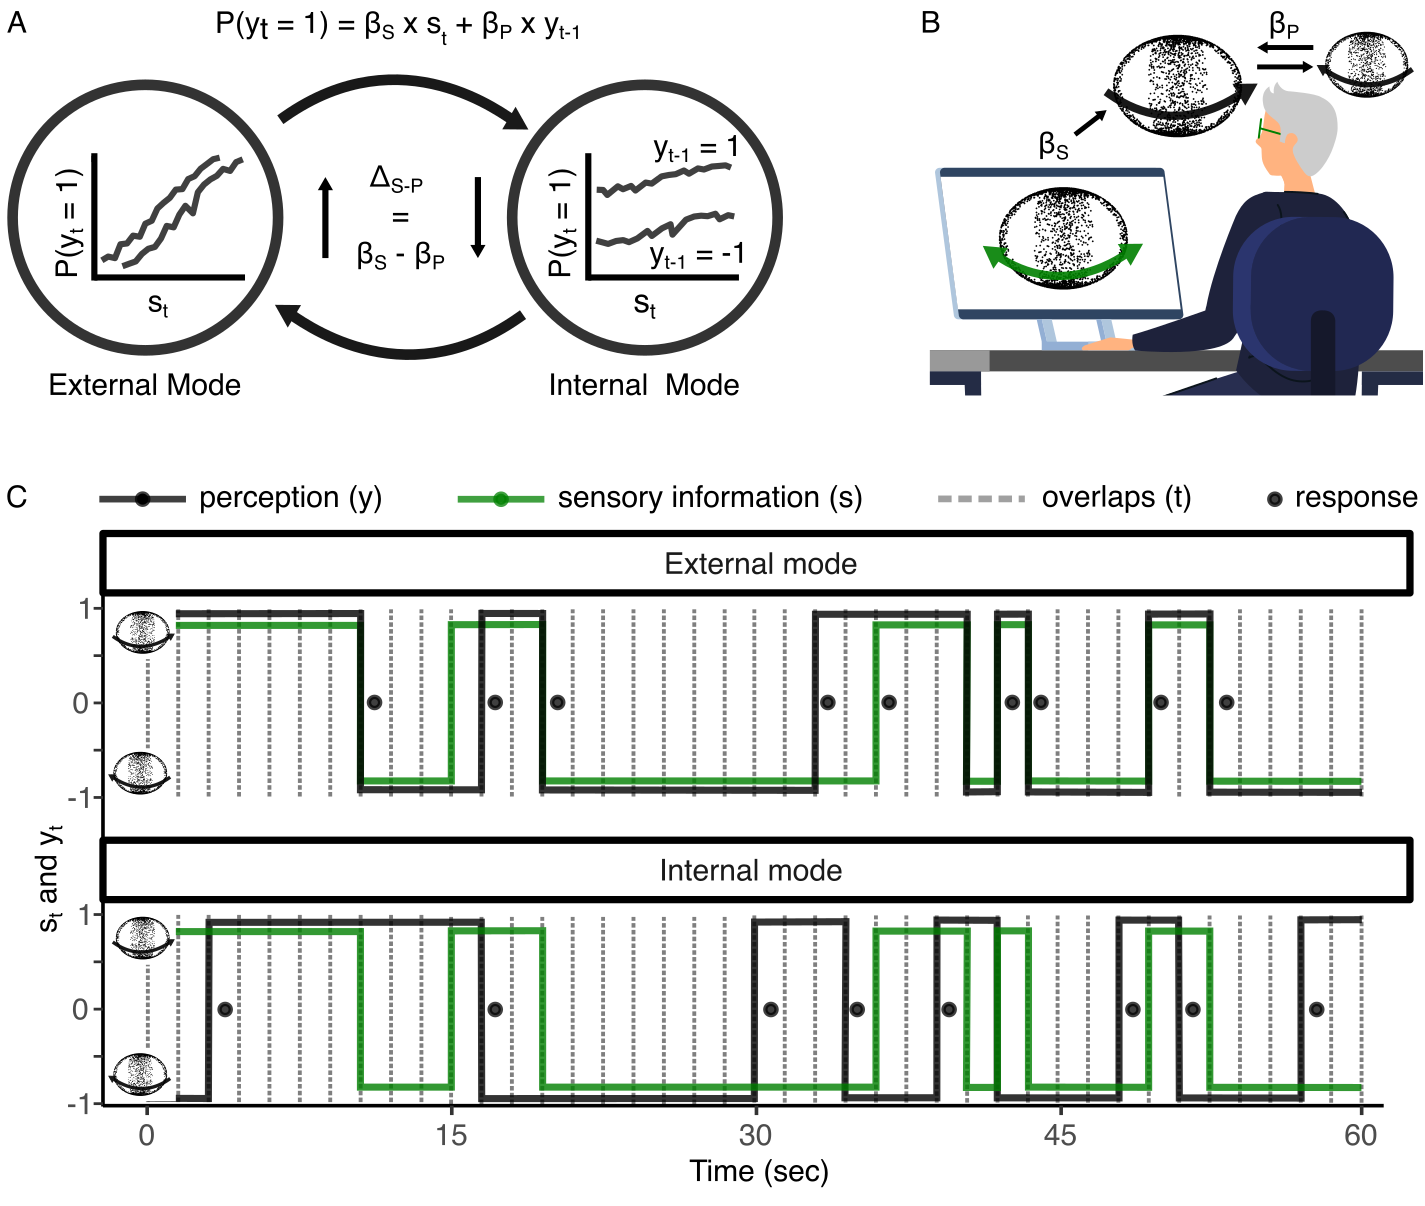
\includegraphics{./modes_ketamine_scz_files/figure-latex/Figure_1.png}

\textbf{Figure 1.}

\textbf{A.} Perception integrates ambiguous sensory signals \(s_t\) with
internal predictions that reflect prior knowledge about the world. One
source of prior knowledge is the temporal autocorrelation of natural
environments, where the recent past often predicts the near future. The
integration of external inputs and internal predictions depends on the
weights assigned to incoming sensory data (\(\beta_S \times s_t\)) and
to internal prediction derived from previous experiences
(\(\beta_P \times y_{t-1}\), dotted versus solid lines, simulated data),
respectively. \(\beta_S\) determines the slope, and \(\beta_P\) the
shift of the psychometric function that links \(s_t\) and \(y_t\).
Importantly, the balance \(\Delta_{S-P} = \beta_S - \beta_P\) is known
to alternate between two opposing modes: During the external mode
(left), perception is largely determined by \(\beta_S \times s_t\),
which is reflected by a steep slope and a small shift of the
psychometric curve. Conversely, during the internal mode (right),
perception is shaped by \(\beta_P \times y_{t-1}\), resulting in a
shallow slope and a large shift of the psychometric curve.

\textbf{B.} We conducted a double-blind placebo-controlled experiment in
28 healthy human participants, who received a continuous infusion with
either the NMDAR antagonist S-ketamine or saline. During the infusion,
the participants viewed SFM stimuli at varying levels of
signal-to-ambiguity (SAR). The stimuli were compatible with two mutually
exclusive subjective experiences (left vs.~rightward rotation of the
front surface, green arrows). Fully ambiguous stimuli (SAR = 0) induce
the phenomenon of bistable perception, where participants perceive
spontaneous changes between the two possible interpretations of the
stimulus (black arrows) at a rate that is governed by \(\beta_P\), the
degree to which perception is shaped by internal predictions derived
from previous experiences. For partially ambiguous stimuli (SAR
\textgreater{} 0), perception reflects the weighted integration of
internal predictions with external sensory data, which is governed by
the balance \(\Delta_{S-P}\) = \(\beta_S\) - \(\beta_P\).

\textbf{C.} Changes in the perceived direction of rotation of the SFM
stimulus occur at brief depth-symmetric configurations of the stimulus
(overlaps, grey dotted lines; Supplemental Video S1). We transformed the
behavioral responses into a sequence of states \(t\) (1.5 sec intervals,
corresponding to the interval between consecutive overlaps), each
associated with a combination of the SAR-weighted input \(s_t\) (green
line) and the perceived direction of rotation \(y_t\) (black line).
Participants reported whenever they experienced a change in conscious
experience (black dots). The response times \(r_t\) was defined as the
lag between the response and the last preceding overlap. We used
HMM-GLMs to quantify the weights \(\beta_S\), \(\beta_P\) and
\(\beta_B\), which reflect how the reported percepts \(y_t\) were
determined by the external inputs \(\beta_S \times s_t\), the internal
predictions \(\beta_P \times y_{t-1}\), and the constant bias
\(\beta_B \times 1\), separately for the external mode (upper panel, 60
sec of example data) and the internal mode (lower panel, 60 sec of
example data with identical \(s(t)\) for visualization). In the external
mode, perception follows the external stimulus closely (high
\(\Delta_{S-P} = \beta_S - \beta_P\)). In the internal mode, perception
is shaped more strongly by internal predictions derived from previous
experiences (low \(\Delta_{S-P}\) = \(\beta_S\) - \(\beta_P\)).

\newpage

\subsection{Figure 2}\label{figure-2}

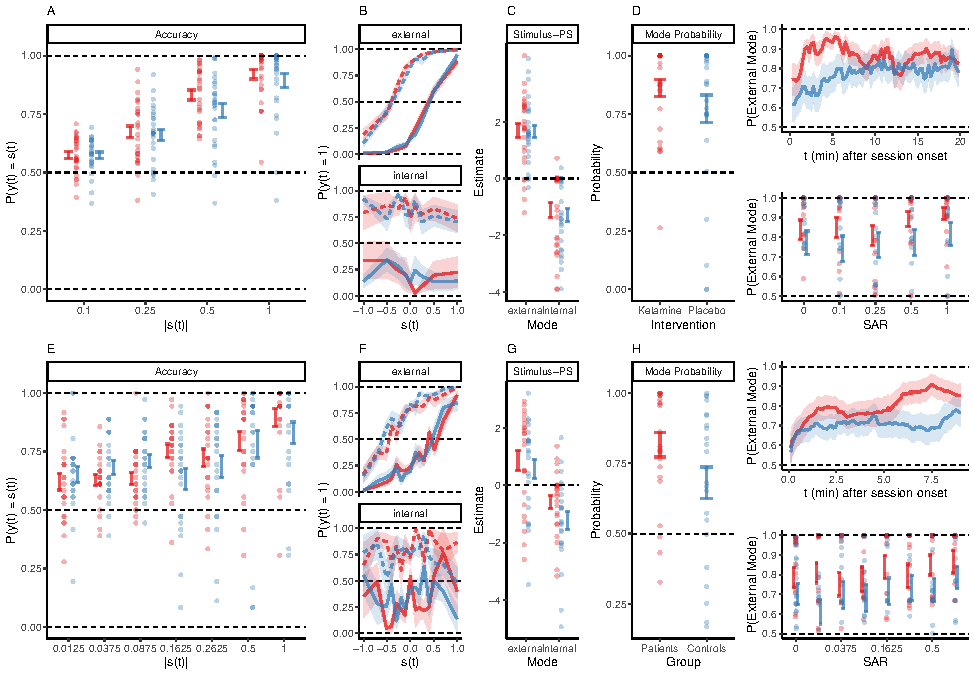
\includegraphics{modes_ketamine_scz_files/figure-latex/Figure_2-1.pdf}

\textbf{Figure 2.}

\textbf{A.} The percepts \(y_t\) were more likely to match the stimuli
\(s_t\) at higher levels of SAR (\(\beta\) = \(3.01\) ± \(0.06\), z =
\(50.39\), p = \(0\)). The positive effect of SAR on
\(P(y_t \cong s_t)\) was more pronounced under S-ketamine (red) relative
to placebo (blue; \(\beta\) = \(0.45\) ± \(0.08\), z = \(5.6\), p =
\(\ensuremath{1.71\times 10^{-7}}\)).

\textbf{B.} In the S-ketamine experiment, the HMM identified two modes
that differed with respect to the relative weighting of external sensory
data and internal predictions: Perception fluctuated between an external
mode, determined by the input \(s_t\) (upper panel panel, steep slope
and small shift of the psychometric curve), and an internal mode,
dominated by a stabilizing prediction that biased perception toward
previous experiences \(y_{t-1}\) (lower panel, shallow slope and large
shift of the psychometric curve). Within modes, there was no significant
effect of S-ketamine (red) versus placebo (blue) on the relation of
\(y(t)\) with \(s(t)\) and \(y(t-1)\).

\textbf{C.} \(\Delta_{S-P}\), the balance between the external input and
the stabilizing internal predictions, was larger during external than
during internal mode (\(\beta\) = \(2.8\) ± \(0.29\), T(\(-81\)) =
\(-9.5\), p = \(\ensuremath{5.22\times 10^{-13}}\)). Importantly, we
found no significant effect of S-ketamine (red) vs.~placebo (blue) on
\(\Delta_{S-P}\) within modes (\(\beta\) = \(-0.03\) ± \(0.29\),
T(\(81\)) = \(-0.1\), p = \(1\)).

\textbf{D.} S-ketamine (red) increased the probability of external mode
(\(\beta\) = \(1.01\) ± \(0.03\), z = \(30.7\), p =
\(\ensuremath{4.26\times 10^{-206}}\)) relative to placebo (blue). The
effect of S-ketamine on mode was present from the start of the session
(\(\beta\) = \(1.77\) ± \(0.07\), z = \(26.9\), p =
\(\ensuremath{3.55\times 10^{-158}}\), upper right panel), with no
significant effect of time (\(\beta\) = \(-0.18\) ± \(0.08\), z =
\(-2.17\), p = \(0.48\)). Relative to placebo, S-ketamine increased the
probability of external mode across all SARs (\(\beta\) = \(0.85\) ±
\(0.06\), z = \(14.14\), p = \(\ensuremath{3.33\times 10^{-44}}\), lower
right panel). Higher SARs were associated with an increased probability
of external mode (\(\beta\) = \(1.34\) ± \(0.09\), z = \(15.01\), p =
\(\ensuremath{9.97\times 10^{-50}}\)), in particular under S-ketamine
(\(\beta\) = \(0.62\) ± \(0.11\), z = \(5.52\), p =
\(\ensuremath{5.27\times 10^{-7}}\)). Alternations between external and
internal mode were found at all SARs: From from full ambiguity to
complete disambiguation, the probability of external mode increased by
only 0.11 under S-ketamine and 0.07 under placebo.

\textbf{E.} In patients (red) and controls (blue), percepts \(y_t\) were
more likely to match the stimuli \(s_t\) at higher levels of SAR
(\(\beta\) = \(2.77\) ± \(0.11\), z = \(24.85\), p =
\(\ensuremath{2.18\times 10^{-135}}\)). Patients followed the external
inputs more closely than controls (\(\beta\) = \(0.75\) ± \(0.15\), z =
\(4.96\), p = \(\ensuremath{5.6\times 10^{-6}}\)).

\textbf{F.} In analogy to the S-ketamine experiment, the HMM identified
two opposing modes in Scz patients (red) and controls (blue). The
external mode increased the sensitivity toward \(s_t\) (slope of the
psychometric function) and weakened the effect of the stabilizing
internal prediction \(y_{t-1}\) (shift between the dotted and solid
line) relative to the internal mode. Within modes, there was no effect
of group on the relation of \(y(t)\) with \(s(t)\) and \(y(t-1)\).

\textbf{G.} The external mode increased \(\Delta_{S-P}\), the balance
between external inputs and internal predictions, in patients (red) and
controls (blue; \(\beta\) = \(1.44\) ± \(0.33\), T(\(44\)) = \(4.33\), p
= \(\ensuremath{3.39\times 10^{-4}}\)), with no significant effect of
group (\(\beta\) = \(-0.28\) ± \(0.54\), T(\(87.97\)) = \(-0.52\), p =
\(1\)).

\textbf{H.} Relative to controls (blue), patients (red) spent more time
in external mode (\(\beta\) = \(0.52\) ± \(0.03\), z = \(16.88\), p =
\(\ensuremath{1.23\times 10^{-63}}\)). In both group, biases toward
external mode increased over time after session onset (\(\beta\) =
\(2.41\) ± \(0.11\), z = \(21.37\), p =
\(\ensuremath{4.07\times 10^{-100}}\); upper right panel), with a
stronger effect in patients (\(\beta\) = \(-1.84\) ± \(0.14\), z =
\(-12.97\), p = \(\ensuremath{2.83\times 10^{-37}}\)). Patients were
more likely than controls to be in external mode across all levels of
SAR (\(\beta\) = \(0.51\) ± \(0.03\), z = \(14.56\), p =
\(\ensuremath{7.57\times 10^{-47}}\), lower right panel). External mode
increased with SAR (\(\beta\) = \(0.63\) ± \(0.1\), z = \(6.47\), p =
\(\ensuremath{1.54\times 10^{-9}}\)), with no significant difference
between groups (\(\beta\) = \(0.15\) ± \(0.13\), z = \(1.16\), p =
\(1\)). As in the S-ketamine experiment, alternations between external
and internal mode were found at all SARs: From from full ambiguity to
complete disambiguation, the probability of external mode increased by
only 0.12 in patients and 0.18 in controls.

\newpage

\section{Supplemental Methods and
Figures}\label{supplemental-methods-and-figures}

\subsection{S-ketamine vs.~placebo}\label{s-ketamine-vs.-placebo}

The S-ketamine experiment consisted in a total of three experimental
sessions. During the first session, we screened participants for
S-ketamine contraindications (arterial hypertension, prior psychiatric
or neurological diagnoses including substance use disorder, use of
psychoactive medication), and assessed psychosis proneness using the
40-item \emph{Peters Delusion Inventory} (PDI\textsuperscript{31}) and
the 32-item \emph{Cardiff Anomalous Perception Scale}
(CAPS\textsuperscript{32}). Moreover, we conducted three experimental
pre-test runs that tested the ability to process stereodisparity (run 1,
SAR = 1, cut-off: perceptual accuracy \textgreater{} 0.75), ensured the
experience of spontaneous switches during bistable perception (run 2,
SAR = 0, cut-off: perceptual stability \textless{} 0.96, corresponding
to phase durations \textless{} 40 sec), and familiarized participants
with the main experiment (run 3, see below for details).

In the subsequent two sessions, participants received a continuous
intravenous infusion of either S-ketamine at 0.1 mg/kg/h or a saline
placebo. Health screenings were repeated before each session to ensure
the participants remained eligible. At each day of testing, we checked
for alcohol intoxication using a breathalyzer and for recent illicit
substance use via a urine drug screen.

Our experimental protocol was double-blinded: The order of S-ketamine
and placebo administration was counter-balanced across participants,
with at least a two week interval between sessions. The participants, as
well as the experimenters tasked with collecting the behavioral and
psychometric data, were unaware of whether S-ketamine or placebo was
administered by an independent group of clinicians who excluded
undiagnosed psychotic illness using the \emph{Brief Psychiatric Rating
Scale} (BPRS\textsuperscript{33}), established the intravenous line,
started the infusion 15 min prior to the experiment, monitored the
participants for side effects (blood pressure, drowsiness, vasovagal
reactions, and psychotomimetic effects), and removed the intravenous
line at the end of the experiment, after which participants were
monitored for at least 30 min. Deblinding occurred after data collection
was complete.

\subsubsection{Sample characteristics}\label{sample-characteristics}

We screened a total of 87 right-handed individuals with (corrected-to-)
normal vision, who were naive to the purpose of the study and gave
written informed consent before participating. All experimental
procedures were approved by the ethics committee at Charité Berlin.

From the group of screened participants, 31 did not meet our pretest
criteria (6 due to perceptual accuracy \textless{} 0.75, 15 due to
perceptual stability \textgreater{} 0.96, 8 due to substance use, 1 due
to do a diagnosis of ADHD, and 1 due to medication with sertraline). Out
of the remaining 56 participants who were eligible for the S-ketamine
experiment, we aborted the main experiment in 1 participant due to high
blood pressure at baseline (RR \textgreater{} 140/80 mmHG), in 2
participants due to strong psychotomimetic effects (micropsia) or
dizziness under S-ketamine, and in 1 participant due to a vasovagal
syncope during intravenous insertion. 24 participants were not available
for the main experiment after successful pre-testing. We therefore
report the data from a total of 28 participants (mean age: 28.93 ± 1.35
years, 18 female) who met all inclusion criteria and completed all
experimental sessions.

\subsubsection{Experimental paradigm}\label{experimental-paradigm}

We presented the experiment using Psychtoolbox 3\textsuperscript{34}
running in Matlab R2021b (session 1: CRT-monitor at 85 Hz, 1280 x 1024
pixels, 60 cm viewing distance and 39.12 pixels per degree visual angle;
session 2 and 32: CRT-monitor at 85Hz, 1280 x 1024 pixels, 40 cm viewing
distance and 26.95 pixels per degree visual angle).

\textbf{Procedure}: Throughout the experiment, participants reported
their perception of a structure-from-motion (SFM) stimulus (Supplemental
Video S1). In this stimulus, random dots distributed on two intersecting
rings induce the perception of a spherical object (diameter: 15.86°,
rotational speed: 12 sec per rotation, rotations per block: 10,
individual dot size: 0.12°) that rotates around a vertical axis with the
front surface to the left or right\textsuperscript{18}. Stimuli were
presented in 120 sec blocks, separated by 10 sec fixation intervals.
Please note that we assessed the participants' perception of the
stimulus based on a fixed response mapping. In our paradigm, perception
and reports are therefore inherently intertwined, with the participants'
reports serving as the sole indicators of their perceptual states.

Participants viewed the stimuli through a custom mirror stereoscope. In
the pretest experiment, we presented stimuli at complete disambiguation
(run 1, SAR = 1), full ambiguity (run 2, SAR = 0) and across five levels
ranging from full ambiguity to complete disambiguation across five
levels (run 3-5, SAR = {[}0, 0.1, 0.25, 0.5, 1{]}). The
signal-to-ambiguity ratio (SAR), which was constant within blocks,
defines the fraction of stimulus dots that carried a disambiguating 3D
signal.

Participants were naive to the potential ambiguity in the visual
display, passively experienced the stimulus and reported changes in
their perception alongside their confidence via button-presses on a
standard USB keyboard (right middle-finger on k: rotation of the
front-surface to the right at high confidence; right index-finger on j:
rotation of the front-surface to the right at low confidence; left
middle-finger on s: rotation of the front-surface to the left at high
confidence; left index-finger on d: rotation of the front-surface to the
left at low confidence; thumb on space bar: unclear direction of
rotation). Unclear perceptual states occurred at a rate of 0.03 ± 0.01
and were excluded from further analyses.

The direction of rotation enforced by \(s_t\) (i.e., whether the
parametric 3D signal enforced leftward or rightward rotation of the
front surface) changed at a rate of 0.15 per overlap (i.e., on average
every 10 sec). Changes in \(s_t\) and the order of blocks, each
corresponding to one level of SAR, were pseudo-random.

In session 1 (pre-test), each run (runs 1 to 3) consisted of six blocks.
In session 2 and 3 (main experiment), each run (run 4 and 5) consisted
of 10 blocks. After every third block, the main experiment was paused to
allow for the monitoring of the participants' vital signs (blood
pressure and pulse rate) and dynamic changes in psychotomimetic
experiences. The latter was assessed using the 6 item
\emph{Clinician-Administered-Dissociative-States-Scale}
(CADSS\textsuperscript{21}) and three additional questions (Q1:
\emph{How awake do you feel?}, Q2: \emph{How intoxicated do you feel?},
Q3: \emph{How nervous do you feel?}) to which participants responded by
clicking on a continuous line that encoded responses from \emph{not at
all} to \emph{very much}. To measure global psychotomimetic effects of
S-ketamine vs.~placebo, participants completed the Questionnaire for the
\emph{Assessment of Altered States of Consciousness}
(5D-ASC\textsuperscript{35}) at the end of session 2 and 3. In addition,
we collected responses on a debriefing questionnaire, in which we asked
participants to describe whether they were able to accurately perceive
the two directions of rotation induced by the SFM stimulus, whether they
noticed any differences between blocks, whether they would guess that
they received S-ketamine or placebo, and whether they had experienced
any effects that they would attribute to a psychoactive substance.

\textbf{Stereodisparity thresholds:} At the beginning of the session 2
and 3, we conducted an independent stereo-acuity test to detect a
potential effect of S-ketamine on stereodisparity
thresholds\textsuperscript{17}. We presented 5000 dots (each at 0.15°
visual angle) within a square of 11° x 11° around a central fixation
cross (0.10°). We added a stereodisparity signal to all dots on a
Landolt C, i.e., a circle (1.37° radius, 2.06° width) with a 90° gap
located either at the left, top, right or bottom. Stimuli were presented
for 1 sec, after which participants reported the location of the gap by
pressing the up-, down-, left- or right-arrow key within a 2 sec
response interval, followed by 5 sec of fixation before the next trial.

We adjusted the stereodisparity of the Landolt C in a two-up-one-down
staircase across 40 trials (initial stereodisparity: 0.0045°, correct
response: decrease in the available stereodisparity by one step;
incorrect response: increase by two steps, initial step-size: 0.001°,
reduction to 0.0005° after first reversal). Stereodisparity thresholds
were defined by the average stereodisparity present at the last 10
trials of the staircase.

\textbf{Scores and Questionnaires:} Supplementary Table S2 provides an
overview of our psychometric data.

\subsection{Scz patients vs.~healthy
controls}\label{scz-patients-vs.-healthy-controls}

To test whether Scz patients show similar changes in perceptual
inference as healthy participants who receive the NMDAR-antagonist
S-ketamine, we re-analyzed data from a previously published case-control
study\textsuperscript{17} that compared Scz patients to healthy
participants in paradigm analogous to the S-ketamine experiment
described above.

\subsubsection{Sample characteristics}\label{sample-characteristics-1}

We report data from 23 patients diagnosed with paranoid Scz (ICD-10:
F20.0, 18 male, age = 37.13±2.42) and 23 controls (17 male, age =
33.57±1.74) that were matched for gender, age and
handedness\textsuperscript{17}.

\subsubsection{Experimental paradigm}\label{experimental-paradigm-1}

Stimuli were presented using Psychtoolbox 3\textsuperscript{34} running
in Matlab R2007b (CRT-Monitor at 60 Hz, 1042x768 pixels, 59.50cm viewing
distance, 30.28 pixels per degree visual angle).

\textbf{Main Experiment}: Throughout the experiment, participants
reported their perception of a SFM stimulus (see Supplemental Video S2)
via button-presses on a standard USB keyboard. In contrast to the
S-ketamine experiment, the 300 dots (0.05°) that composed the stimulus
(2.05°x 2.05°) were not placed on rings, but on a Lissajous band defined
by the perpendicular intersection of two sinusoids (\(x(p) = sin(A*p)\)
and \(y(p) = cos(B*p + \delta\)) with A=3, B=6, with \(\delta\)
increasing from 0 to \(2\pi\) at 0.15 Hz. Overlapping configurations of
the stimulus occurred in intervals of 3.33 sec.~Participants viewed the
stimuli through a mirror stereoscope. Fusion was supported by
rectangular fusion-frames and a background of random dot noise (700 dots
of 0.05° which moved at a speed of 1.98° per sec and changed their
direction at a rate of 1 Hz).

We presented participants with 3 sessions of the main experiment, each
consisting of 14 40.08 sec blocks that were separated by 5 sec of
fixation and differed with respect to the SAR, ranging from full
ambiguity to complete disambiguation in 8 levels (SAR = {[}0, 0.01,
0.04, 0.9, 0.16, 0.26, 0.50, 1{]}). The frequency of changes in the
direction of the disambiguating signal corresponded to the frequency of
spontaneous changes that participants perceived during full
ambiguity\textsuperscript{17} (SAR = 0). In contrast to the S-ketamine
experiment, participants only reported the perceived direction of
rotation \(y_t\) (left vs.~rightward movement of the front surface),
with no additional assessment of confidence.

\textbf{Stereodisparity thresholds:} We measured stereodisparity
thresholds in Scz patients and controls using the procedure described
above.

\textbf{Scores and Questionnaires:} We used the PDI\textsuperscript{31}
and the CAPS\textsuperscript{32} to measure delusional ideation and
perceptual anomalies in Scz patients and controls. Clinical symptom
severity was assessed using the \emph{Positive and Negative Syndrome
Scale} (PANSS)\textsuperscript{36}.

\subsection{Quantification and statistical
procedures}\label{quantification-and-statistical-procedures}

This manuscript was written in RMarkdown. All data and summary
statistics can be reviewed by cloning the Github respository
\url{https://github.com/veithweilnhammer/modes_ketamine_scz} and running
the file \emph{modes\_ketamine\_scz.Rmd}.

The SFM stimuli used in the above studies share an important feature:
Even though physically ambiguous at all angles of rotation, spontaneous
changes in the perceived direction of rotation are limited to
overlapping configurations of the stimuli\textsuperscript{17,18} (see
also Supplemental Figure S2 and S4). This is because depth-symmetry,
which is a prerequisite for changes in subjective experiences during
bistable SFM\textsuperscript{17,18}, is limited to timepoints when the
bands that compose the stimuli overlap (Supplemental Video S1 and S2).

We therefore discretized the perceptual timecourse of all experiments
into a sequence of overlaps that occur at times t (1.5 sec inter-overlap
interval for the S-ketamine intervention, 3.33 sec inter-overlap
interval for the case-control study). We characterized each
inter-overlap interval the primary independent variable \(s_t\) = {[}-1,
1{]} \(\times\) SAR (the SAR-weighted input ranging from maximum
information for leftward rotation to maximum information for rightward
rotation), and \(y_{t-1}\) (the perceptual experience associated with
the preceding overlap). As secondary independent variables, we
considered block and session index (reflecting the time participants
were exposed to the experiment), participant identifiers and, if
applicable, treatment or group identifiers. Primary dependent variables
were \(y_t\) = {[}0,1{]} (the experience of either leftward or rightward
rotation) and, if applicable, \(c_t\) = {[}0,1{]} (low vs.~high
confidence). As secondary dependent variables, we computed perceptual
accuracy (the probability of \(y_t \cong s_t\)) and perceptual stability
(the probability of \(y_t = y(t - 1)\)).

From the perspective of predictive processing, perceptual stability is
induced by internal predictions that bias perception toward previous
experiences\textsuperscript{19}. Stabilizing internal predictions are
most likely to be adaptive in natural environments, where the recent
past predicts the near future (much like successive frames captured by a
video camera are temporarily autocorrelated\textsuperscript{19}). Our
experiment differed from the temporal autocorrelation of natural
environments\textsuperscript{19} in that random changes in the direction
of disambiguation (i.e., whether the external stimulus supports left- or
rightward rotation of the sphere) occurred in average intervals of 10
sec.~We thereby created a situation in which strong stabilizing internal
predictions \emph{reduce} performance\textsuperscript{38}. In our
experiment, a shift of perception away from internal predictions toward
the external sensory data, which has been proposed to occur under
S-ketamine and in Scz\textsuperscript{1}, should therefore manifest as
an \emph{increase} in perceptual accuracy.

For SFM stimuli like those used in this study, changes in experience
occur at overlapping configurations of the
stimulus\textsuperscript{17,18,39,40} (i.e., when the bands that compose
the stimulus overlap; see Supplemental Video S1-2). Following previous
approaches\textsuperscript{17,18,40}, we defined response times \(r_t\)
as the time between a button press that indicates a change in the
perceived direction of rotation and the time of the preceding
overlapping configuration of the stimulus (see Figure 1C).

To assess differences in metacognitive performance, we correlated
perceptual confidence with perceptual accuracy. We computed meta-d', a
measure of metacognitive sensitivity that indicates how well confidence
ratings predict perceptual accuracy\textsuperscript{41}.

For all variables, we report and display averages as mean ± standard
error of the mean (s.e.m).

\subsubsection{Conventional statistics}\label{conventional-statistics}

The goal of our conventional statistics was to quantify the effect of
NMDAR hypofunction, whether due to pharmacological antagonism with
S-ketamine or due to a diagnosis of Scz, on the interpretation of
ambiguous sensory information. We performed standard logistic and linear
regression by fitting (general) mixed linear effects models using the
R-packages lmer, glmer and afex (see Supplemental Table S2). We
predicted \(y_t\), \(c_t\), perceptual accuracy and perceptual stability
in logistic regression, and \(r_t\) in linear regression. We estimated
random intercepts defined within participants in the S-ketamine
experiment and nested random intercepts for participants within groups
in the case-control study. We applied a Bonferroni-correction for the
number of main effects and interactions within models. Mixed effects
models are reported with the estimate (\(\beta\) without subscript),
followed by the T- or z-statistic for linear and logistic models,
respectively. Please note that parameter estimates with subscripts refer
exclusively to the GLM-HMM weights (see Computational modeling)
associated with the external input (\(\beta_S\)), the constant bias
(\(\beta_B\)), and the previous experience (\(\beta_P\)). For
non-normally distributed secondary dependent variables, we performed
rank-based tests to assess correlations (Spearman) and distribution
differences (Wilcoxon).

\subsubsection{Computational modeling}\label{computational-modeling}

Having established the effect of NMDAR hypofunction on the
interpretation of ambiguous sensory information, we used computational
modeling to arbitrate between two mechanistic explanations on how
S-ketamine and Scz may alter perceptual inference.

\textbf{Hypothesis H1: Unimodal inference.} In one scenario, NMDAR
hypofunction may induce a global increase in the sensitivity to external
inputs relative to stabilizing internal predictions. This unimodal
scenario, which corresponds to the canocical predictive processing
hypothesis of Scz\textsuperscript{1}, assumes S-ketamine- or Scz-related
changes in the weights \(w \equiv \{\beta_S, \beta_P, \beta_B\}\) of a
GLM that predicts percepts \(y_t\) from the input vector \(x_t\), which
consists in the SAR-weighted external input \(s_t\), the stabilizing
internal prediction \(y_{t-1}\) and a constant bias b:

\[
P(y_t = 1 | x_t) = \frac{1}{1 + e^{-x_t \times w}} 
\]

\[
x_t \times w =  s_t \times \beta_S + y_{t-1} \times \beta_P  + b \times \beta_B  
\]

According to the unimodal hypothesis H1, NMDAR hypofunction increases
\(\beta_S\) at the expense of \(\beta_P\), leading to an increase of
\(\Delta_{S-P}\) = \(\beta_S\) - \(\beta_P\).

\textbf{Hypothesis H2: Bimodal inference.} In an alternative scenario,
NMDAR hypofunction does not change the weights of the GLM directly, but
modulates the transition between latent modes\textsuperscript{15} or
decision-making strategies\textsuperscript{14} that differ with respect
to the balance between external inputs \(s_t\) and the stabilizing
internal prediction provided by \(y_{t-1}\). In the bimodal scenario,
perceptual inference is characterized by two latent modes \(z_t\) (i.e.,
states in a HMM) that alternate at a probability per overlap that is
defined by a 2 x 2 transition matrix \(A\):

\[
P(z_t = k|z_{t-1} = j) = A_{kj} 
\]

Each state \(z_t\) is associated by an independent GLM defined by the
weights \(w_k\):

\[
P(y_t = 1 | x_t, z_t) = \frac{1}{1 + e^{-x_t \times w_k}} 
\]

\[
x_t \times w_k =  s_t \times \beta_{S,k} + y_{t-1} \times \beta_{P,k}  + b \times \beta_{B,k}  
\]

Hypothesis H2 differs from the unimodal hypothesis H1 in two ways:
First, the two-state GLM-HMM is characterized by two (as opposed to one)
GLMs that differ with respect to \(\Delta_{S-P}\): In the external mode,
\(\beta_S\) is increased relative to \(\beta_P\). Conversely, in the
internal mode, \(\beta_P\) is increased relative to \(\beta_S\). Second,
during bimodal inference, NMDAR hypofunction does not alter the weights
within the external and internal GLMs, but modulates the transition
probability between the two.

\textbf{Procedure:} To contrast hypotheses H1 and H2, we fitted unimodal
and bimodal GLM-HMMs using SSM\textsuperscript{42} (Supplemental Table
S2), compared models via Bayesian Information Criterion (BIC), and
assessed the effects of S-ketamine or Scz on the posterior model
parameters, i.e., HMM transition probabilities and the mode-dependent
GLM weights \(w_k\). Model fitting using SSM is governed by the
hyperparameters \(\sigma^2\) and \(\alpha\). \(\sigma^2\) denotes the
variance of a prior over the GLM weights \(w_k\). Smaller values of
\(\sigma^2\) shrink \(w_k\) toward 0, whereas \(\sigma\) = \(\infty\)
leads to flat priors. We set \(\sigma^2\) to 100 for GLMs that predicted
group-level data, and to 1 for GLMs that predicted participant- or
session-level data, which were initialized with group-level estimates of
\(w_k\). \(\alpha\) defines the Dirichlet prior over the transition
matrix \(A\) and is flat for \(\alpha\) = 1. We set \(\alpha\) to 1 for
all group-level and participant-level fits.

For each experiment, computational modeling was carried out in a
sequence of 3 steps: In a first step, we fitted a unimodal GLM
initialized with noisy weights to the group-level data (i.e., data
pooled across participants within an individual experiment) for a total
of n = 100 iterations and computed the average posterior weights
\(w_n\). In a second step, we fitted the group-level data with the
unimodal and the bimodal GLM-HMM initialized by \(w_n\), extracted the
posterior parameters \(w_k\), and compared the models using BIC.

In a third step, we fitted the unimodal and the bimodal GLM-HMM to
session-level data (S-ketamine experiment) and participant-level data
(case-control experiment). Models were initialized by the average
weights \(w_n\) of the corresponding group-level model. For all bimodal
group-, participant- and session-level GLM-HMMs, we defined the latent
mode associated with the higher posterior \(\beta_S\) estimate as
external. For summary statistics, we extracted the posterior weights
\(w_k\) (separately for external and internal mode) and the dynamic
posterior probability of external mode \(z_t = e\).

The GLM-HMM used in this study predicts experiences \(y_t\) in a GLM
defined by the stimulus \(s_t\), the preceding experience \(y_{t-1}\),
and a constant bias b. The HMM component of the model identifies
alternations between two states that differ with respect to the weights
of any combination of \(s_t\), \(y_{t-1}\), and b. We used the GLM-HMM
to test our primary hypothesis that ketamine and Scz alter the balance
between two states that differ with respect to \(\Delta_{S-P}\) =
\(\beta_S\) - \(\beta_P\) (high \(\Delta_{S-P}\) in external mode, low
\(\Delta_{S-P}\) in internal mode: hypothesis H2). However, the GLM-HMM
can, in principle, embody dynamic changes in any combination of
\(\beta_S\), \(\beta_B\), and \(\beta_P\). Alternative outcomes to
external versus internal modes are states that differ with respect to
bias (state 1: high \(\beta_B\); state 2: low \(\beta_B\); hypothesis
H3) and randomness (state 1: high \(\beta_S\) and \(\beta_P\); state 2:
low \(\beta_S\) and \(\beta_P\): no difference in \(\Delta_{S-P}\)
between modes: hypothesis H4).

\textbf{Stimulus- versus experienced-based GLM-HMM.} In our experiment,
stabilizing internal predictions bias perception toward preceding
overlaps (t-1), causing conflicts between the direction of rotation that
is consciously experienced (y) and the stimuli s presented at the
current overlap t. If external and internal modes are perceptual in
nature, then the stabilization of perception should be driven by the
sequence of perceptual experiences y, as opposed to the sequence of
sensory signals s (hypothesis H5). To test this hypothesis, we compared
our \emph{experienced-based} GLM-HMM, in which the stabilizing internal
predictions are driven by the participants' perceptual experience at the
preceding overlap, with an alternative \emph{stimulus-based} GLM, in
which the stabilizing internal predictions are driven by the stimulus
presented at the preceding overlap.

\textbf{External validation of the GLM-HMM.} The GLM-HMM generates a
perceptual decision variable \(P(y_t = 1)\) that is defined by a
weighted integration of the external stimulus (\(\beta_S \times s_t\)),
the previous experience (\(\beta_P \times y_{t-1}\)), and a constant
bias (\(\beta_P \times 1\)). The weights are obtained by fitting the
GLM-HMM to the sequence of experiences \(y\), irrespective of whether
the experience \(y\) was made at high or low confidence. This allowed us
to test whether the predictions of the two-state GLM-HMM would
generalize to metacognitive reports on perception. Importantly, the
source of confidence differs between the modes: During the external
mode, confidence should depend predominantly on the SAR of the stimulus.
Conversely, during the internal mode, confidence should be driven more
by the congruency of perception with previous experiences, and less by
the external input. To validate our model, we tested whether the
perceptual decision variable \(P(y_t = 1)\) predicted not only the
binary contents of experience \(y_t\) (which the GLM-HMM was fitted to),
but also perceptual confidence \(c_t\) (which the GLM-HMM was not fitted
to). To do so, we correlated \(c_t\) (as reported by the participants)
with the posterior certainty \(C_t\) (as provided by the GLM-HMM) at
each overlap. The posterior certainty \(C_t\) is given by log
probability of the actual experience \(y\), given the decision variable
\(P(y_t = 1)\):

\[
C_t = y_t \cdot \log(P(y_t = 1)) + (1 - y_t) \cdot \log(1 - P(y_t = 1)) 
\]

Please note that the interpretation of our results is inherently limited
to the hypotheses incorporated in the above GLMs. In our paradigm,
behavioral reports at the time of changes in experience served as the
only indicators of the perceptual and metacognitive states of the
participants. These behavioral reports were collected with a fixed
stimulus-response mapping, such that the GLM-based analyses cannot fully
separate perception and response behavior.

\textbf{Recovery of GLM-HMM parameters.} To evaluate the robustness of
our GLM-HMM model in estimating mode-dependent weights and transition
probabilities, we conducted a parameter recovery analysis. The GLM-HMM
is characterized by three weights, \(\beta_S\), \(\beta_B\), and
\(\beta_P\), that are defined separately for the external and internal
modes. We assessed the model's ability to estimate individual
mode-dependent weights by fitting the model to simulated data that were
obtained by sampling from GLM-HMMs in which individual target weights
were systematically varied, while all other weights were kept constant
at the group-level average obtained from the original data. For each
analysis, we selected one of the six weights (3 weights \(\times\) 2
modes) and varied its value parametrically from -1 to 5. We then
generated synthetic data, simulating \(y_{\text{syn}}\) for n = 78400
overlaps (corresponding to the number of overlaps observed across all
participants in the S-ketamine experiment). The GLM-HMM model was then
fitted to these synthetic data.

We repeated the recovery analysis for each weight 10 times, computed the
average posterior weights \(\beta_S\), \(\beta_B\), and \(\beta_P\), and
then correlated these recovered weights with the synthetic input
weights. We applied a similar procedure to evaluate the recovery of the
GLM-HMM transition matrix. Transition probabilities were varied
parametrically within the range of 0.8 to 1 for on-diagonal cells
(external to external, internal to internal) and 0 to 0.2 for
off-diagonal cells (external to internal, internal to external). The
results of this recovery analysis, which are depicted in Supplemental
Figure S1, demonstrate that the GLM-HMM weights and transition
probabilities can be recovered with high fidelity across the full range
of the synthetic input parameters, and in particular in the parameter
region of the group-level estimates obtained from the original data
(\(w_n\)).

\subsection{Supplemental Figure S1}\label{supplemental-figure-s1}

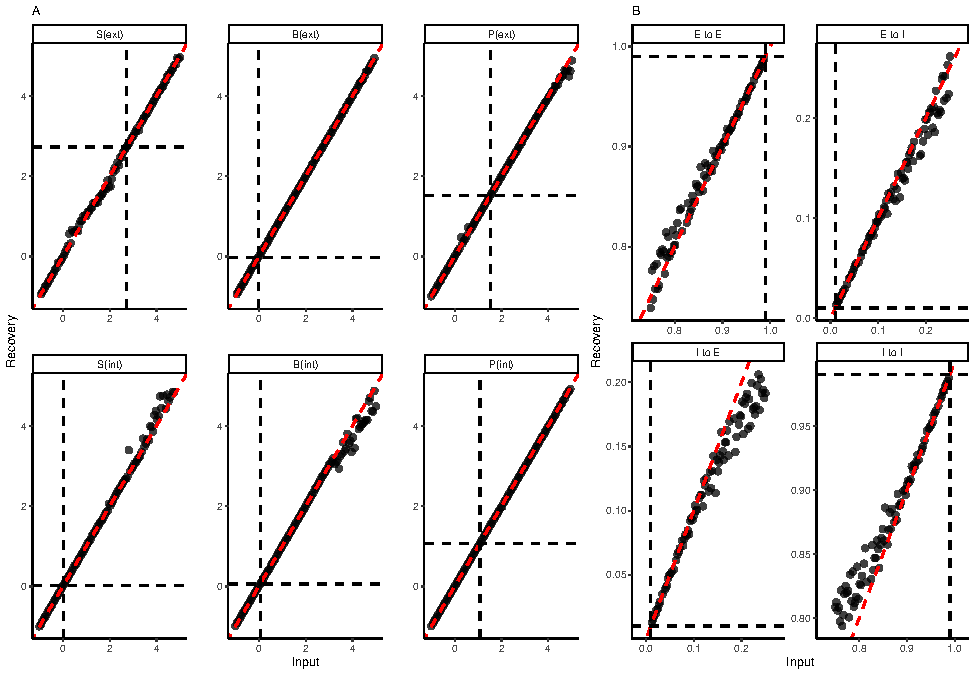
\includegraphics{modes_ketamine_scz_files/figure-latex/Supplemental_Figure_S1-1.pdf}
\textbf{Supplemental Figure S1. GLM-HMM parameter recovery}

\textbf{A. Weight recovery from simulated data: GLM weights.} The
GLM-HMM is defined by the mode-dependent weights \(\beta_S\),
\(\beta_B\), and \(\beta_P\). To test how well our GLM-HMM can recover
changes in individual weights, we selected one of the six weights (3
weights x 2 modes) and varied its value parametrically from -1 to 5. For
each inversion, we kept all other weights at the group-level average
obtained from the original data. For each of the six recovery analyses,
we simulated synthetic experiences \(y_{syn}\) for n = 78400 overlaps
(number of overlaps across participants in the S-ketamine experiment).
We then fitted a randomly initialized GLM-HMM to the synthetic
experiences, and extracted the weights recovered from the synthetic
experiences \(y_{syn}\). We performed each recovery for 10 iterations,
computed the average posterior weights \(\beta_S\), \(\beta_B\), and
\(\beta_P\), and correlated them with the synthetic input weights. The
correlation with the parametric input weights and the posterior weights
recovered from the simulated data were close to 1 for all weights
(\(\beta_S\), \(\beta_B\), and \(\beta_P\), columns) and modes (external
and internal, rows). Weights were recovered with high fidelity across a
broad range of weights (average r = 0.99), and in particular at the
group-level weights \(w_n\) obtained from the original data (black
dotted line). The red dashed line represents the identity line (slope =
1, intercept = 0), indicating perfect recovery.

\textbf{B. Weight recovery from simulated data: transition matrix.} We
repeated the above procedure for each cell of the GLM-HMM transition
matrix. We initialized models with parametric transition probabilities
ranging from 0.8 to 1 (on-diagonal cells, external to external, internal
to internal) and 0 to 0.2 (off-diagonal cells, external to internal,
internal to external). Transition probabilities were recovered with high
fidelity across a broad range of parameters (average r = 0.99), and in
particular at the group-level estimates obtained from the original data
(black dotted line). The red dashed line represents the identity line
(slope = 1, intercept = 0), indicating perfect recovery.

\newpage

\subsection{Supplemental Figure S2}\label{supplemental-figure-s2}

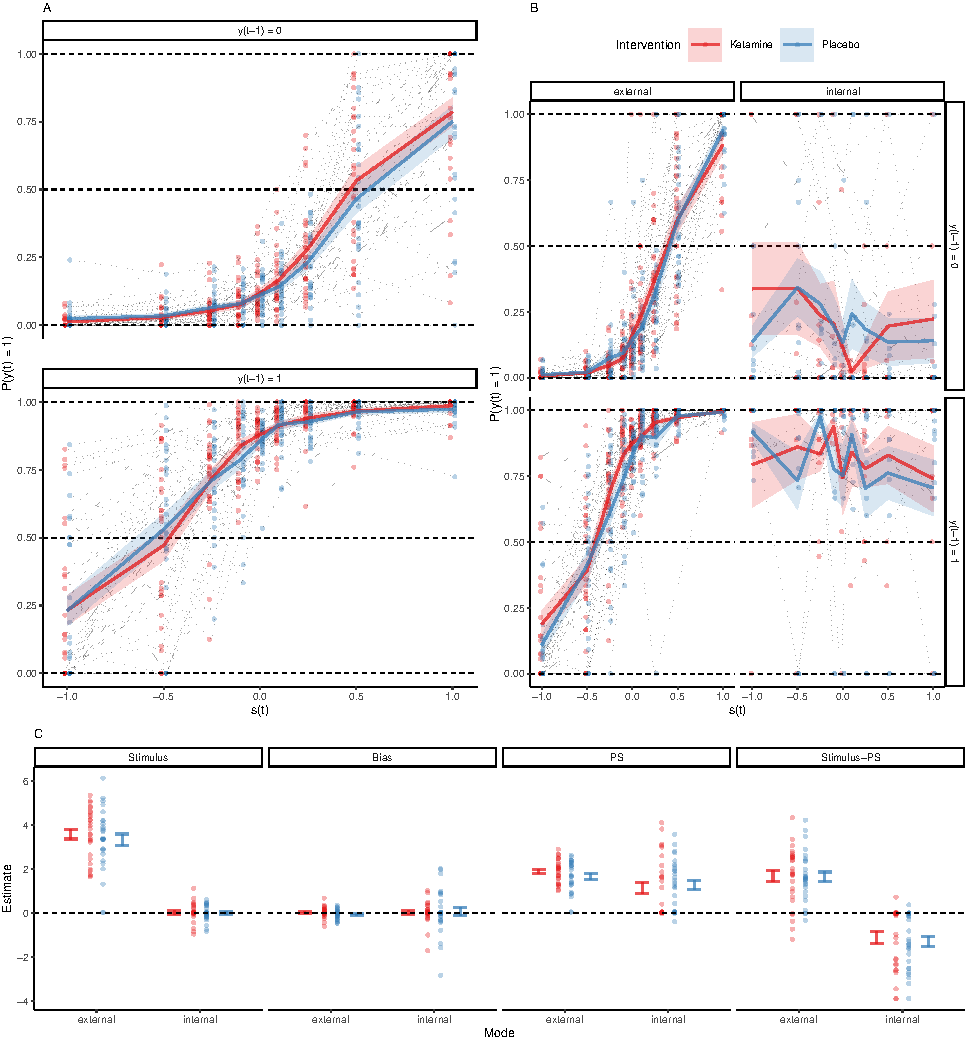
\includegraphics{modes_ketamine_scz_files/figure-latex/Supplemental_Figure_S2-1.pdf}

\textbf{Supplemental Figure S2. The effects of ketamine and bimodal
inference on RT.}

\textbf{A.} RT were non-uniformly distributed across the inter-overlap
interval (D = \(0.09\), p = \(\ensuremath{5.38\times 10^{-9}}\),
one-sample Kolmogorov-Smirnov test). This corroborates that changes in
perception aligned with the overlapping configurations of the stimulus
after S-ketamine (red) and placebo (blue).

\textbf{B.} RT showed a quadratic relationship with \(s_t\) (\(\beta\) =
\(-6.87\) ± \(1.68\), T(\(\ensuremath{6.2\times 10^{3}}\)) = \(-4.1\), p
= \(\ensuremath{5.1\times 10^{-4}}\)), indicating faster responses when
sensory information was reliable (\(|s_t| \gg  0\); note that SAR as
shown in Figure 2A and 2E is equal to \(|s_t|\)). We observed no main
effect of S-ketamine (red) vs.~placebo (blue) on RT (\(\beta\) =
\(\ensuremath{-3.35\times 10^{-3}}\) ± \(0.01\),
T(\(\ensuremath{6.2\times 10^{3}}\)) = \(-0.32\), p = \(1\)).

\textbf{C.} We found no additional effect of mode on RT (\(\beta\) =
\(0.02\) ± \(0.03\), z = \(\ensuremath{5.96\times 10^{3}}\), p =
\(0.78\)).

\textbf{D.} Confidence showed a quadratic relationship with \(s_t\)
(\(\beta\) = \(74.83\) ± \(2.39\), z = \(31.32\), p =
\(\ensuremath{3.22\times 10^{-214}}\)), confirming that participants
were more confident when sensory information was reliable
(\(|s_t| = SAR \gg  0\)). Relative to placebo (blue), S-ketamine (red)
reduced choice confidence (\(\beta\) = \(-0.21\) ± \(0.04\), z =
\(-5.9\), p = \(\ensuremath{4.36\times 10^{-8}}\)), and decreased the
quadratic effect of \(s_t\) on confidence (\(\beta\) = \(-19.95\) ±
\(2.36\), z = \(-8.45\), p = \(\ensuremath{3.48\times 10^{-16}}\)).

\textbf{E.} External mode increased confidence globally (\(\beta\) =
\(0.72\) ± \(0.07\), z = \(9.92\), p =
\(\ensuremath{7.85\times 10^{-22}}\)) and by elevating the quadratic
effect of \(s_t\) on confidence (\(\beta\) = \(242.61\) ± \(18.43\), z =
\(13.16\), p = \(\ensuremath{3.37\times 10^{-38}}\)). When controlling
for mode, the negative effect of S-ketamine (red) vs.~placebo (blue) on
confidence and on the quadratic relationship of confidence with \(s_t\)
remained significant.

\newpage

\subsection{Supplemental Figure S3}\label{supplemental-figure-s3}

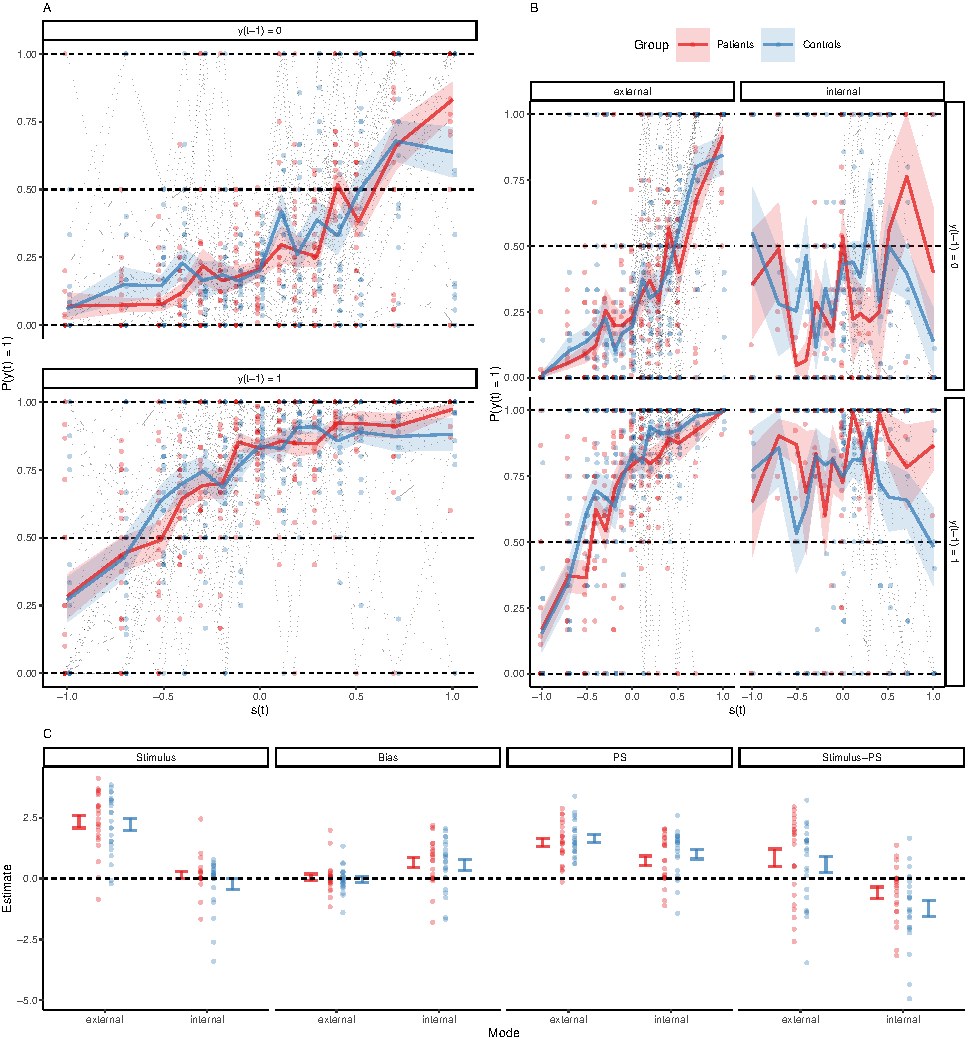
\includegraphics{modes_ketamine_scz_files/figure-latex/Supplemental_Figure_S3-1.pdf}

\textbf{Supplemental Figure S3. Extended data on the effects of
S-ketamine and mode on perceptual inference (related to Figure 2A-C).}

\textbf{A.} Here, we show psychometric curves (percept \(y_t\) versus
input \(s_t\)) under S-ketamine (red) and placebo (blue). The plot
separates times \(t\) for which the previous experience was leftward
rotation (\(y_{t-1} = -1\), upper panel) and rightward rotation
(\(y_{t-1} = +1\), lower panel). As expected, \(y_t\) was driven by both
the external input \(s_t\) (\(\beta_S\) = \(3.01\) ± \(0.06\), z =
\(50.39\), p = \(0\)) and the previous percept \(y_{t-1}\)
(\(\beta_{P}\) = \(2.06\) ± \(0.03\), z = \(80.58\), p = \(0\)). We
found no significant interaction between the \(s_t\) and \(y_{t-1}\)
(\(\beta\) = \(-0.06\) ± \(0.06\), z = \(-1.06\), p = \(1\)). Relative
to placebo, S-ketamine caused a shift of \(y_t\) toward \(s_t\)
(\(\beta\) = \(0.45\) ± \(0.08\), z = \(5.6\), p =
\(\ensuremath{1.71\times 10^{-7}}\)), with no significant effect on
\(y_{t-1}\) (\(\beta\) = \(0.08\) ± \(0.04\), z = \(2.39\), p =
\(0.13\)). We found no significant three-way-interaction (drug x \(s_t\)
x \(y_{t-1}\), \(\beta\) = \(-0.07\) ± \(0.08\), z = \(-0.9\), p =
\(1\)).

\textbf{B.} This panel shows the data from panel (A) separately for
times \(t\) where the HMM identified the mode of perceptual inference as
external (left panels) or internal (right panels). When the mode of
perceptual processing was added to the prediction of \(y_t\) from
\(s_t\) and \(y_{t-1}\), the effect S-ketamine (red) vs.~placebo (blue)
on \(s_t\) disappeared (\(\beta\) = \(0.24\) ± \(0.11\), z = \(2.13\), p
= \(0.53\)). Instead, changes in the balance between \(s_t\) and
\(y_{t-1}\) were loaded onto fluctuations between external and internal
mode, which caused perception to shift away from external inputs \(s_t\)
(\(\beta\) = \(-4.23\) ± \(0.21\), z = \(-20.01\), p =
\(\ensuremath{7.54\times 10^{-88}}\)) and toward previous experiences
\(y{t-1}\) (\(\beta\) = \(0.78\) ± \(0.09\), z = \(8.64\), p =
\(\ensuremath{8.81\times 10^{-17}}\)).

\textbf{C.} Here, we plot the weights from the GLM
\(y_t = \beta_S \times s_t + \beta_P \times y_{t-1} + \beta_B \times 1\),
alongside the balance between external inputs and previous experiences
\(\Delta_{S-P} = \beta_S - \beta_P\) during external and internal mode.
Colors indicate S-ketamine (red) and placebo (blue). \(\beta_S\), the
weight associated with the external input \(s_t\), was positive in
external mode, but reduced to zero in internal mode (\(\beta\) =
\(-3.55\) ± \(0.23\), T(\(81\)) = \(-15.44\), p =
\(\ensuremath{4.78\times 10^{-24}}\)). We found no additional effect of
S-ketamine (red) versus placebo (blue; \(\beta\) = \(-0.25\) ± \(0.23\),
T(\(81\)) = \(-1.1\), p = \(1\)) and no significant interaction
(\(\beta\) = \(0.21\) ± \(0.33\), T(\(81\)) = \(0.65\), p = \(1\)).
\(\beta_B\), the weight associated with the constant response bias \(b\)
toward rightward rotation, was not different from zero (\(\beta_B\) =
\(0.04\) ± \(0.11\), T(\(98.36\)) = \(0.31\), p = \(1\)). We found no
effect of drug (\(\beta\) = \(-0.11\) ± \(0.14\), T(\(81\)) = \(-0.74\),
p = \(1\)) or mode (\(\beta\) = \(-0.02\) ± \(0.14\), T(\(81\)) =
\(-0.12\), p = \(1\)) on the bias weight \(\beta_B\). \(\beta_P\), the
weight associated with the previous percept \(y_{t-1}\) was not
modulated by S-ketamine (\(\beta\) = \(-0.22\) ± \(0.26\), T(\(81\)) =
\(-0.87\), p = \(1\)) or mode (\(\beta\) = \(-0.75\) ± \(0.26\),
T(\(81\)) = \(-2.92\), p = \(0.29\)). There was no significant
interaction between drug and mode with respect to \(\beta_P\) (\(\beta\)
= \(0.35\) ± \(0.36\), T(\(81\)) = \(0.97\), p = \(1\)). The balance
\(\Delta_{S-P}\) between external inputs and internal predictions was
determined by mode (\(\beta\) = \(2.8\) ± \(0.29\), T(\(81\)) = \(9.5\),
p = \(\ensuremath{5.22\times 10^{-13}}\)), with no significant effect of
S-ketamine (\(\beta\) = \(0.03\) ± \(0.29\), T(\(81\)) = \(0.1\), p =
\(1\)) and no interaction (\(\beta\) = \(0.14\) ± \(0.42\), T(\(81\)) =
\(0.34\), p = \(1\)). These posterior GLM-HMM weights argue against the
alternative hypotheses that the primary effect of S-ketamine is related
to changes in dynamics of bias (state 1: high \(\beta_B\); state 2: low
\(\beta_B\); hypothesis H3) or the randomness of experience (state 1:
high \(\beta_S\) and \(\beta_P\); state 2: low \(\beta_S\) and
\(\beta_P\) with no difference in \(\Delta_{S-P}\) between modes:
hypothesis H4).

\textbf{D.} S-ketamine (red) increased the probability of external mode
(\(\beta\) = \(1.01\) ± \(0.03\), z = \(30.7\), p =
\(\ensuremath{4.26\times 10^{-206}}\)) relative to placebo (blue) by
elevating the stability of external at the expense of internal mode (EE
versus II; left panels; V = 264, p = 0.01), with no effect on the
transition probabilities between modes (EI versus IE; right panels; V =
149, p = 0.37).

\newpage

\subsection{Supplemental Figure S4}\label{supplemental-figure-s4}

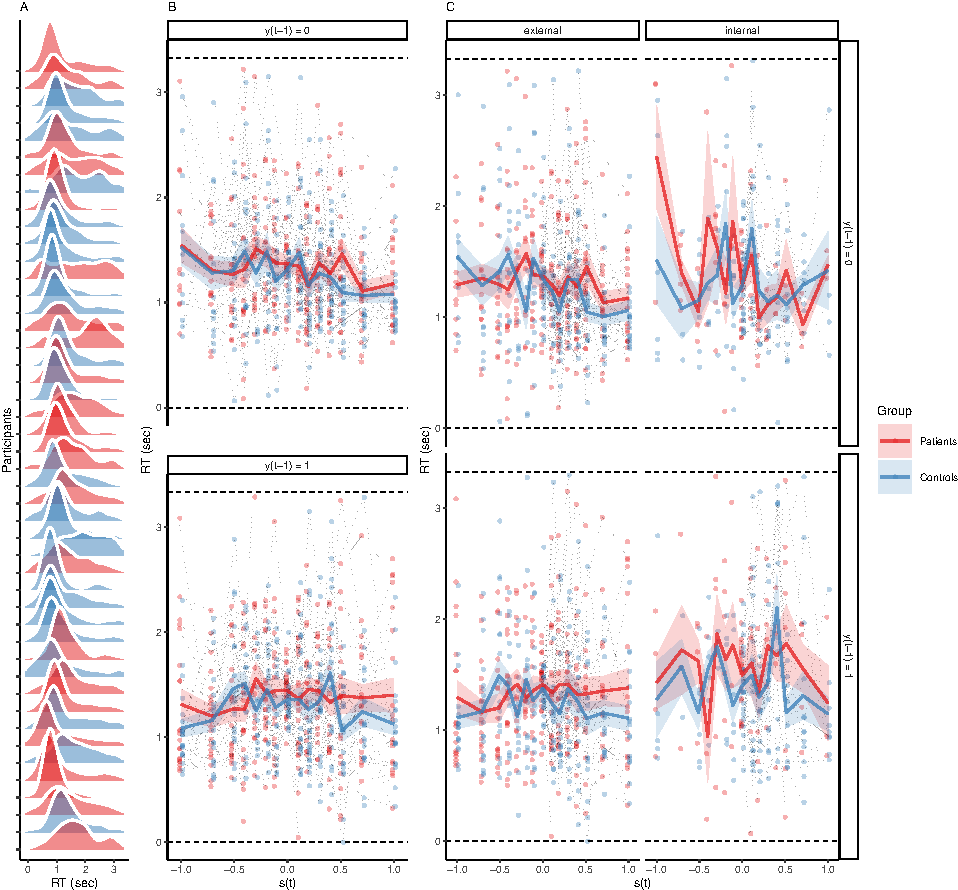
\includegraphics{modes_ketamine_scz_files/figure-latex/Supplemental_Figure_S4-1.pdf}

\textbf{Supplemental Figure S4. Extended data on external and internal
mode in Scz patients and healthy controls (related to Figure 2E-H).}

\textbf{A.} Here, we show psychometric curves (percept \(y_t\) versus
input \(s_t\)) in patients (red) and controls (blue). The plot separates
times \(t\) for which the previous experience was leftward rotation
(\(y_{t-1} = -1\), upper panel) and rightward rotation
(\(y_{t-1} = +1\), lower panel). Perception was driven by \(s_t\)
(\(\beta_S\) = \(2.77\) ± \(0.11\), z = \(24.85\), p =
\(\ensuremath{2.18\times 10^{-135}}\)) and \(y_{t-1}\) (\(\beta_{P}\) =
\(1.5\) ± \(0.03\), z = \(58.2\), p = \(0\)), with no significant
interaction between \(s_t\) and \(y_{t-1}\) (\(\beta\) =
\(\ensuremath{-5.41\times 10^{-3}}\) ± \(0.11\), z = \(-0.05\), p =
\(1\)). Patients were more sensitive to \(s_t\) (\(\beta\) = \(0.75\) ±
\(0.15\), z = \(4.96\), p = \(\ensuremath{5.6\times 10^{-6}}\)). We
found no significant three-way-interaction (group x \(s_t\) x
\(y_{t-1}\), \(\beta\) = \(-0.37\) ± \(0.15\), z = \(-2.45\), p =
\(0.11\)).

\textbf{B.} This panel shows the data from panel (A) separately for
times \(t\) where the HMM identified the mode of perceptual inference as
external (left panels) or internal (right panels). When the mode of
perceptual processing was added to the prediction of \(y_t\) from
\(s_t\) and \(y_{t-1}\), the difference between patients (red) and
controls (blue) in the effect of \(s_t\) on \(y_t\) disappeared
(\(\beta\) = \(-0.02\) ± \(0.22\), z = \(-0.08\), p = \(1\)). Instead,
changes in the balance between \(s_t\) and \(y_{t-1}\) were loaded onto
fluctuations between external and internal mode, which caused perception
to shift away from external inputs \(s_t\) (\(\beta\) = \(-3.47\) ±
\(0.29\), z = \(-11.95\), p = \(\ensuremath{1.01\times 10^{-31}}\)) and
toward previous experiences \(y{t-1}\) (\(\beta\) = \(0.5\) ± \(0.07\),
z = \(6.85\), p = \(\ensuremath{1.15\times 10^{-10}}\)).

\textbf{C.} Here, we plot the weights from the GLM
\(y_t = \beta_S \times s_t + \beta_P \times y_{t-1} + \beta_B \times 1\),
alongside the balance between external inputs and previous experiences
\(\Delta_{S-P} = \beta_S - \beta_P\) during external and internal mode.
Colors indicate the group (patients in red, controls in blue).
\(\beta_S\), the weight associated with the external input \(s_t\), was
positive in external mode, but reduced to zero in internal mode
(\(\beta\) = \(-2.19\) ± \(0.24\), T(\(44\)) = \(-9.13\), p =
\(\ensuremath{4.07\times 10^{-11}}\)). We found no additional effect of
group (\(\beta\) = \(-0.11\) ± \(0.37\), T(\(87.69\)) = \(-0.3\), p =
\(1\)) and no significant interaction (\(\beta\) = \(-0.25\) ± \(0.34\),
T(\(44\)) = \(-0.74\), p = \(1\)). \(\beta_B\), the weight associated
with the constant response bias \(b\) toward rightward rotation, was not
different from zero (\(\beta\) = \(0.05\) ± \(0.18\),
T(\(\ensuremath{1.62\times 10^{-8}}\)) = \(0.29\), p = \(1\)). We found
no effect of group (\(\beta\) = \(-0.09\) ± \(0.25\),
T(\(\ensuremath{1.62\times 10^{-8}}\)) = \(-0.37\), p = \(1\)). There
was a trend for a positive effect of internal mode (\(\beta\) = \(0.6\)
± \(0.24\), T(\(88\)) = \(2.47\), p = \(0.06\)) on the bias weight
\(\beta_B\). \(\beta_P\), the weight associated with the previous
percept \(y_{t-1}\), was reduced in internal mode (\(\beta\) = \(-0.75\)
± \(0.26\), T(\(88\)) = \(-2.92\), p = \(0.02\)), but not modulated by
group (\(\beta\) = \(0.17\) ± \(0.32\),
T(\(\ensuremath{9.88\times 10^{-10}}\)) = \(0.54\), p = \(1\)). There
was no significant interaction between group and mode with respect to
\(\beta_P\) (\(\beta\) = \(0.11\) ± \(0.36\), T(\(88\)) = \(0.3\), p =
\(1\)). The balance \(\Delta_{S-P}\) between external inputs and
internal predictions was determined by mode (\(\beta\) = \(1.44\) ±
\(0.33\), T(\(81\)) = \(9.5\), p = \(\ensuremath{3.39\times 10^{-4}}\)),
with no significant effect of group (\(\beta\) = \(0.28\) ± \(0.54\),
T(\(87.97\)) = \(0.52\), p = \(1\)) and no interaction (\(\beta\) =
\(0.36\) ± \(0.47\), T(\(44\)) = \(0.76\), p = \(1\)). These posterior
GLM-HMM weights argue against the alternative hypotheses that the
primary effect of S-ketamine is related to changes in dynamics of bias
(state 1: high \(\beta_B\); state 2: low \(\beta_B\); hypothesis H3) or
the randomness of experience (state 1: high \(\beta_S\) and \(\beta_P\);
state 2: low \(\beta_S\) and \(\beta_P\) with no difference in
\(\Delta_{S-P}\) between modes: hypothesis H4).

\textbf{D.} Relative to controls (blue), patients (red) spent more time
in external mode (\(\beta\) = \(0.52\) ± \(0.03\), z = \(16.88\), p =
\(\ensuremath{1.23\times 10^{-63}}\)). This effect was driven by an
increase in the stability of external mode at the expense of internal
mode (EE versus II; left panels; W = 352, p = 0.03). There was no effect
of group on the transition probabilities between modes (EI versus IE;
right panels; W = 248, p = 0.65).

\newpage

\subsection{Supplemental Figure S5}\label{supplemental-figure-s5}

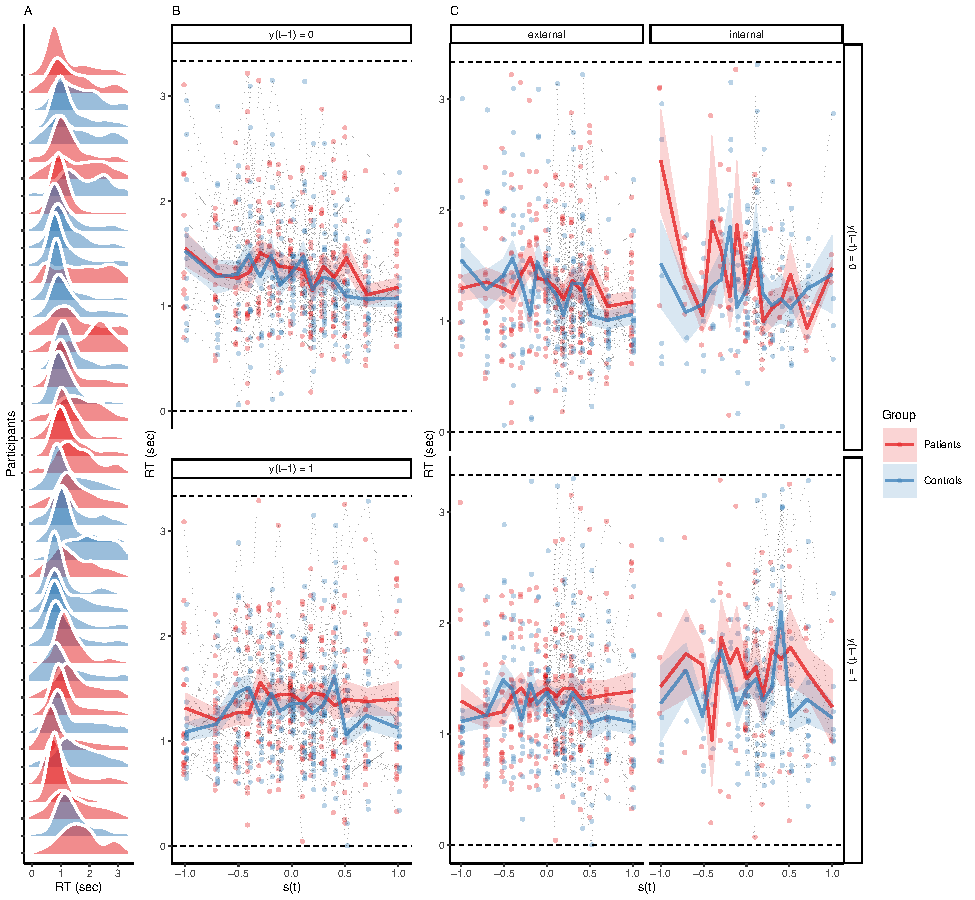
\includegraphics{modes_ketamine_scz_files/figure-latex/Supplemental_Figure_S5-1.pdf}

\textbf{Supplemental Figure S5. RT and bimodal inference in Scz patients
and controls.}

\textbf{A.} RT were non-uniformly distributed across the inter-overlap
interval (D = \(0.22\), p = \(\ensuremath{2.39\times 10^{-232}}\),
one-sample Kolmogorov-Smirnov test against uniformity) in patients (red)
and controls (blue). This confirmed that changes in perception were
aligned with the overlapping configurations of the stimulus.

\textbf{B.} RT did not differ between patients (red) and controls (blue;
\(\beta\) = \(-0.07\) ± \(0.08\), T(\(66.96\)) = \(-0.87\), p = \(1\)).
We found no quadratic relationship between RT and \(s_t\) (\(\beta\) =
\(-3.54\) ± \(2.34\), T(\(\ensuremath{5.33\times 10^{3}}\)) = \(-1.51\),
p = \(1\)).

\textbf{C.} We found no effect of mode on RT (\(\beta\) = \(0.03\) ±
\(0.04\), z = \(\ensuremath{4.89\times 10^{3}}\), p = \(0.76\)).

\newpage

\subsection{Supplemental Figure S6}\label{supplemental-figure-s6}

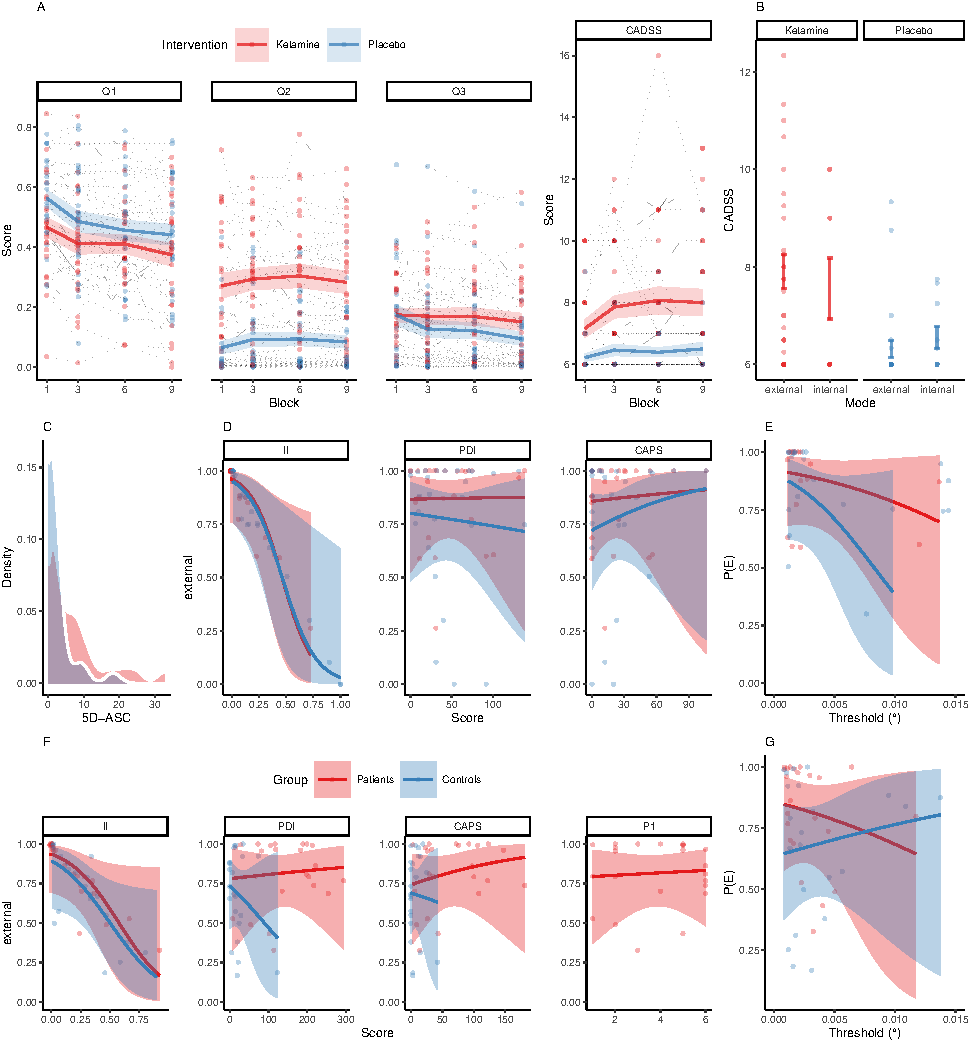
\includegraphics{modes_ketamine_scz_files/figure-latex/Supplemental_Figure_S6-1.pdf}

\textbf{Supplemental Figure S6. Scores and Questionnaires.}

\textbf{A.} Responses to Q1 (\emph{How awake do you feel?}) indicated
that participants felt more tired under S-ketamine (red) than placebo
(blue; \(\beta\) = \(-1.53\) ± \(0.6\), z = \(-2.57\), p = \(0.04\)),
with no significant effect of time or a between-factor interaction.
Responses to Q2 (\emph{How intoxicated do you feel?}) indicated that
participants felt more intoxicated under S-ketamine (\(\beta\) =
\(3.32\) ± \(1.44\), z = \(2.3\), p = \(0.09\)), with no significant
effect of time or a between-factor interaction. Responses to Q3
(\emph{How nervous do you feel?}) revealed no effect of S-ketamine
(\(\beta\) = \(-3.01\) ± \(2.62\), z = \(-1.15\), p = \(1\)), time, nor
a significant between-factor interaction. CADSS scores were elevated
under S-ketamine (\(\beta\) = \(1.01\) ± \(0.34\), T(\(185.32\)) =
\(2.99\), p = \(0.01\)) with a borderline trend for an increase over
time (\(0.09\) ± \(0.04\), T(\(185.61\)) = \(2.24\), p = \(0.1\)) and no
significant between-factor interaction.

\textbf{B.} Q1-3 and CADSS scores were collected after blocks 1, 3, 6
and 9. To assess how the mode of perceptual inference was linked to
dissociative symptoms, we separated the participants ratings according
to the mode that dominated perception at the very end of the preceding
block. While controlling the effect of S-ketamine (red) vs placebo
(blue), we found that external mode increased dissociative symptoms
(\(\beta\) = \(1.05\) ± \(0.54\), T(\(208.05\)) = \(1.95\), p =
\(0.05\)), but had no effect on wakefulness (Q1), subjective
intoxication (Q2) or nervousness (Q3).

\textbf{C.} 5-ASC scores were elevated under S-ketamine (red) relative
to placebo (blue; \(\beta\) = \(4.89\) ± \(1.59\), T(\(27.14\)) =
\(3.08\), p = \(\ensuremath{9.33\times 10^{-3}}\)).

\textbf{D.} Neither PDI, CAPS, nor 5-ASC scores were predictive of the
probability of external mode (shown separately for S-ketamine in red and
placebo in blue).

\textbf{E.} Stereodisparity thresholds were not predictive of the
probability of external mode (\(\beta\) = \(-28.73\) ± \(781.1\), z =
\(-0.04\), p = \(0.97\)). Thresholds did not differ between S-ketamine
(red) and placebo (blue; W = \(102\), p = \(0.66\)).

\textbf{F.} Neither PDI, CAPS (patients in red and controls in blue),
nor the PANSS items P1 (delusions) or P3 (hallucinations, patients only)
predicted the probability of external mode.

\textbf{G.} In patients (red) and controls (blue), stereodisparity
thresholds were not predictive of the probability of external mode
(\(\beta\) = \(-1.88\) ± \(2.05\), z = \(-0.92\), p = \(1\)). Thresholds
did not differ between groups (V = \(976\), p = \(0.52\)).

\newpage

\subsection{Supplemental Table S1}\label{supplemental-table-s1}

\begin{longtable}[]{@{}
  >{\raggedright\arraybackslash}p{(\columnwidth - 4\tabcolsep) * \real{0.3148}}
  >{\raggedright\arraybackslash}p{(\columnwidth - 4\tabcolsep) * \real{0.4537}}
  >{\raggedright\arraybackslash}p{(\columnwidth - 4\tabcolsep) * \real{0.2315}}@{}}
\toprule\noalign{}
\begin{minipage}[b]{\linewidth}\raggedright
RESOURCE
\end{minipage} & \begin{minipage}[b]{\linewidth}\raggedright
SOURCE
\end{minipage} & \begin{minipage}[b]{\linewidth}\raggedright
IDENTIFIER
\end{minipage} \\
\midrule\noalign{}
\endhead
\bottomrule\noalign{}
\endlastfoot
\textbf{Deposited data \& code} & & \\
Analyzed data \& custom code &
\url{https://github.com/veithweilnhammer/modes_ketamine_scz/} & N/A \\
\textbf{Software} & & \\
\textbf{Matlab} & \url{https://www.mathworks.com/} & RRID:SCR\_001622 \\
Psychtoolbox 3 & \url{http://psychtoolbox.org/} & RRID:SCR\_002881 \\
\textbf{R} & \url{http://www.r-project.org/} & RRID:SCR\_001905 \\
RStudio & \url{https://www.rstudio.com/} & RRID:SCR\_000432 \\
lme4, afex, statConfR, ggplot2, ggridges, gridExtra, tidyr, plyr, readxl
& \url{http://cran.r-project.org/} & RRID:SCR\_003005 \\
\textbf{Python 3} & \url{http://www.python.org/} & RRID:SCR\_008394 \\
Jupyter Notebook & \url{https://jupyter.org/} & RRID:SCR\_018315 \\
numpy & \url{http://www.numpy.org} & RRID:SCR\_008633 \\
pandas & \url{https://pandas.pydata.org} & RRID:SCR\_018214 \\
SSM & \url{https://github.com/lindermanlab/ssm} & N/A \\
\end{longtable}

\textbf{Supplemental Table S1. Key resources.}

\newpage

\subsection{Supplemental Table S2}\label{supplemental-table-s2}

\begin{longtable}[]{@{}
  >{\raggedright\arraybackslash}p{(\columnwidth - 6\tabcolsep) * \real{0.1818}}
  >{\raggedright\arraybackslash}p{(\columnwidth - 6\tabcolsep) * \real{0.4364}}
  >{\raggedright\arraybackslash}p{(\columnwidth - 6\tabcolsep) * \real{0.1818}}
  >{\raggedright\arraybackslash}p{(\columnwidth - 6\tabcolsep) * \real{0.2000}}@{}}
\toprule\noalign{}
\begin{minipage}[b]{\linewidth}\raggedright
Scale
\end{minipage} & \begin{minipage}[b]{\linewidth}\raggedright
Scope
\end{minipage} & \begin{minipage}[b]{\linewidth}\raggedright
Condition
\end{minipage} & \begin{minipage}[b]{\linewidth}\raggedright
mean ± s.e.m.
\end{minipage} \\
\midrule\noalign{}
\endhead
\bottomrule\noalign{}
\endlastfoot
\textbf{PDI}\textsuperscript{31} & Delusion proneness & Global & 46.22 ±
7.19 \\
\textbf{CAPS}\textsuperscript{32} & Hallucination proneness & Global &
23 ± 5.05 \\
\textbf{BPRS}\textsuperscript{33} & Screen for psychotic illness &
Global & 0.64 ± 0.27 \\
\textbf{5D-ASC}\textsuperscript{35} & Altered states of consciousness &
S-ketamine & 7.11 ± 1.59 \\
& & Placebo & 2.2 ± 0.75 \\
\textbf{CADSS}\textsuperscript{21} & Dissociation & S-ketamine & 7.8 ±
0.33 \\
& & Placebo & 6.43 ± 0.17 \\
\textbf{Q1} & Wakefulness & S-ketamine & 0.41 ± 0.03 \\
& & Placebo & 0.48 ± 0.03 \\
\textbf{Q2} & Intoxication & S-ketamine & 0.29 ± 0.03 \\
& & Placebo & 0.09 ± 0.02 \\
\textbf{Q3} & Nervousness & S-ketamine & 0.17 ± 0.02 \\
& & Placebo & 0.13 ± 0.03 \\
\textbf{Stereovision} & Disparity thresholds & S-ketamine &
\ensuremath{2.89\times 10^{-3}} ± \ensuremath{6.18\times 10^{-4}} \\
& & Placebo & \ensuremath{2.75\times 10^{-3}} ±
\ensuremath{4.39\times 10^{-4}} \\
\end{longtable}

\textbf{Supplemental Table S2. Psychometric data for the S-ketamine
experiment.}

\newpage

\subsection{Supplemental Table S3}\label{supplemental-table-s3}

\begin{longtable}[]{@{}
  >{\raggedright\arraybackslash}p{(\columnwidth - 6\tabcolsep) * \real{0.1818}}
  >{\raggedright\arraybackslash}p{(\columnwidth - 6\tabcolsep) * \real{0.4364}}
  >{\raggedright\arraybackslash}p{(\columnwidth - 6\tabcolsep) * \real{0.1818}}
  >{\raggedright\arraybackslash}p{(\columnwidth - 6\tabcolsep) * \real{0.2000}}@{}}
\toprule\noalign{}
\begin{minipage}[b]{\linewidth}\raggedright
Scale
\end{minipage} & \begin{minipage}[b]{\linewidth}\raggedright
Scope
\end{minipage} & \begin{minipage}[b]{\linewidth}\raggedright
Condition
\end{minipage} & \begin{minipage}[b]{\linewidth}\raggedright
mean ± s.e.m.
\end{minipage} \\
\midrule\noalign{}
\endhead
\bottomrule\noalign{}
\endlastfoot
\textbf{PDI}\textsuperscript{31} & Delusion proneness & Patients &
138.83 ± 16.64 \\
& & Controls & 21.87 ± 5.75 \\
\textbf{CAPS}\textsuperscript{32} & Hallucination proneness & Patients &
65.17 ± 10.56 \\
& & Controls & 7.13 ± 2.2 \\
\textbf{P1} & Delusions & Patients & 3.83 ± 0.39 \\
\textbf{P3} & Delusions & Patients & 3.35 ± 0.44 \\
\textbf{Stereovision} & Disparity thresholds & Patients &
\ensuremath{2.82\times 10^{-3}} ± \ensuremath{5.13\times 10^{-4}} \\
& & Controls & \ensuremath{3.46\times 10^{-3}} ±
\ensuremath{7.14\times 10^{-4}} \\
\end{longtable}

\textbf{Supplemental Table S3. Psychometric data for Scz-control-study.}

\newpage

\section*{References}\label{references}
\addcontentsline{toc}{section}{References}

\phantomsection\label{refs}
\begin{CSLReferences}{0}{0}
\bibitem[\citeproctext]{ref-Sterzer2018}
\CSLLeftMargin{1. }%
\CSLRightInline{Sterzer, P. \emph{et al.}
\href{https://doi.org/10.1016/j.biopsych.2018.05.015}{The {Predictive}
{Coding} {Account} of {Psychosis}}. \emph{Biological Psychiatry}
\textbf{84}, 634--643 (2018).}

\bibitem[\citeproctext]{ref-Friston2005}
\CSLLeftMargin{2. }%
\CSLRightInline{Friston, K.
\href{https://doi.org/10.1098/rstb.2005.1622}{A theory of cortical
responses.} \emph{Philosophical transactions of the Royal Society of
London. Series B, Biological sciences} \textbf{360}, 815--836 (2005).}

\bibitem[\citeproctext]{ref-Rao1999}
\CSLLeftMargin{3. }%
\CSLRightInline{Rao, R. P. \emph{et al.}
\href{https://doi.org/10.1038/4580}{Predictive coding in the visual
cortex: A functional interpretation of some extra-classical
receptive-field effects.} \emph{Nature neuroscience} \textbf{2}, 79--87
(1999).}

\bibitem[\citeproctext]{ref-feldman_attention_2010}
\CSLLeftMargin{4. }%
\CSLRightInline{Feldman, H. \emph{et al.}
\href{https://doi.org/10.3389/FNHUM.2010.00215/BIBTEX}{Attention,
uncertainty, and free-energy}. \emph{Frontiers in Human Neuroscience}
\textbf{4}, 7028 (2010).}

\bibitem[\citeproctext]{ref-muthukumaraswamy_evidence_2015}
\CSLLeftMargin{5. }%
\CSLRightInline{Muthukumaraswamy, S. D. \emph{et al.}
\href{https://doi.org/10.1523/JNEUROSCI.0903-15.2015}{Evidence that
{Subanesthetic} {Doses} of {Ketamine} {Cause} {Sustained} {Disruptions}
of {NMDA} and {AMPA}-{Mediated} {Frontoparietal} {Connectivity} in
{Humans}}. \emph{Journal of Neuroscience} \textbf{35}, 11694--11706
(2015).}

\bibitem[\citeproctext]{ref-corlett_glutamatergic_2011}
\CSLLeftMargin{6. }%
\CSLRightInline{Corlett, P. R. \emph{et al.}
\href{https://doi.org/10.1038/npp.2010.163}{Glutamatergic {Model}
{Psychoses}: {Prediction} {Error}, {Learning}, and {Inference}}.
\emph{Neuropsychopharmacology} \textbf{36}, 294--315 (2011).}

\bibitem[\citeproctext]{ref-Stein2020}
\CSLLeftMargin{7. }%
\CSLRightInline{Stein, H. \emph{et al.}
\href{https://doi.org/10.1038/s41467-020-18033-3}{Reduced serial
dependence suggests deficits in synaptic potentiation in anti-{NMDAR}
encephalitis and schizophrenia}. \emph{Nature Communications}
\textbf{11}, 1--11 (2020).}

\bibitem[\citeproctext]{ref-murray_linking_2014}
\CSLLeftMargin{8. }%
\CSLRightInline{Murray, J. D. \emph{et al.}
\href{https://doi.org/10.1093/cercor/bhs370}{Linking {Microcircuit}
{Dysfunction} to {Cognitive} {Impairment}: {Effects} of {Disinhibition}
{Associated} with {Schizophrenia} in a {Cortical} {Working} {Memory}
{Model}}. \emph{Cerebral Cortex} \textbf{24}, 859--872 (2014).}

\bibitem[\citeproctext]{ref-catts_quantitative_2016}
\CSLLeftMargin{9. }%
\CSLRightInline{Catts, V. S. \emph{et al.}
\href{https://doi.org/10.1016/j.biopsycho.2015.10.013}{A quantitative
review of the postmortem evidence for decreased cortical
{N}-methyl-{D}-aspartate receptor expression levels in schizophrenia:
{How} can we link molecular abnormalities to mismatch negativity
deficits?} \emph{Biological Psychology} \textbf{116}, 57--67 (2016).}

\bibitem[\citeproctext]{ref-adams_computational_2022}
\CSLLeftMargin{10. }%
\CSLRightInline{Adams, R. A. \emph{et al.}
\href{https://doi.org/10.1016/j.biopsych.2021.07.024}{Computational
{Modeling} of {Electroencephalography} and {Functional} {Magnetic}
{Resonance} {Imaging} {Paradigms} {Indicates} a {Consistent} {Loss} of
{Pyramidal} {Cell} {Synaptic} {Gain} in {Schizophrenia}}.
\emph{Biological Psychiatry} \textbf{91}, 202--215 (2022).}

\bibitem[\citeproctext]{ref-self_different_2012}
\CSLLeftMargin{11. }%
\CSLRightInline{Self, M. W. \emph{et al.}
\href{https://doi.org/10.1073/pnas.1119527109}{Different glutamate
receptors convey feedforward and recurrent processing in macaque {V1}}.
\emph{Proceedings of the National Academy of Sciences} \textbf{109},
11031--11036 (2012).}

\bibitem[\citeproctext]{ref-castro-alamancos_short-term_1996}
\CSLLeftMargin{12. }%
\CSLRightInline{Castro-Alamancos, M. A. \emph{et al.}
\href{https://doi.org/10.1073/pnas.93.3.1335}{Short-term synaptic
enhancement and long-term potentiation in neocortex.} \emph{Proceedings
of the National Academy of Sciences} \textbf{93}, 1335--1339 (1996).}

\bibitem[\citeproctext]{ref-nakazawa_spatial_2017}
\CSLLeftMargin{13. }%
\CSLRightInline{Nakazawa, K. \emph{et al.}
\href{https://doi.org/10.1038/s41537-016-0003-3}{Spatial and temporal
boundaries of {NMDA} receptor hypofunction leading to schizophrenia}.
\emph{npj Schizophrenia} \textbf{3}, 1--11 (2017).}

\bibitem[\citeproctext]{ref-ashwood_mice_2022}
\CSLLeftMargin{14. }%
\CSLRightInline{Ashwood, Z. C. \emph{et al.}
\href{https://doi.org/10.1038/s41593-021-01007-z}{Mice alternate between
discrete strategies during perceptual decision-making}. \emph{Nature
Neuroscience} \textbf{25}, 201--212 (2022).}

\bibitem[\citeproctext]{ref-weilnhammer_sensory_2023}
\CSLLeftMargin{15. }%
\CSLRightInline{Weilnhammer, V. \emph{et al.}
\href{https://doi.org/10.1371/journal.pbio.3002410}{Sensory processing
in humans and mice fluctuates between external and internal modes}.
\emph{PLOS Biology} \textbf{21}, e3002410 (2023).}

\bibitem[\citeproctext]{ref-albert_hierarchical_2017}
\CSLLeftMargin{16. }%
\CSLRightInline{Albert, S. \emph{et al.}
\href{https://doi.org/10.1371/journal.pcbi.1005856}{A hierarchical
stochastic model for bistable perception}. \emph{PLOS Computational
Biology} \textbf{13}, e1005856 (2017).}

\bibitem[\citeproctext]{ref-weilnhammer_psychotic_2020}
\CSLLeftMargin{17. }%
\CSLRightInline{Weilnhammer, V. \emph{et al.}
\href{http://www.ncbi.nlm.nih.gov/pubmed/32090246}{Psychotic
{Experiences} in {Schizophrenia} and {Sensitivity} to {Sensory}
{Evidence}.} \emph{Schizophrenia bulletin} \textbf{46}, 927--936
(2020).}

\bibitem[\citeproctext]{ref-weilnhammer_active_2021}
\CSLLeftMargin{18. }%
\CSLRightInline{Weilnhammer, V. \emph{et al.}
\href{https://doi.org/10.1016/j.cub.2021.04.043}{An active role of
inferior frontal cortex in conscious experience}. \emph{Current Biology}
\textbf{31}, 2868--2880.e8 (2021).}

\bibitem[\citeproctext]{ref-manassi_continuity_2024}
\CSLLeftMargin{19. }%
\CSLRightInline{Manassi, M. \emph{et al.}
\href{https://doi.org/10.1038/s44159-024-00297-x}{Continuity fields
enhance visual perception through positive serial dependence}.
\emph{Nature Reviews Psychology} \textbf{3}, 352--366 (2024).}

\bibitem[\citeproctext]{ref-shergill_evidence_2005}
\CSLLeftMargin{20. }%
\CSLRightInline{Shergill, S. S. \emph{et al.}
\href{https://doi.org/10.1176/appi.ajp.162.12.2384}{Evidence for sensory
prediction deficits in schizophrenia}. \emph{The American Journal of
Psychiatry} \textbf{162}, 2384--2386 (2005).}

\bibitem[\citeproctext]{ref-mertens_clinician-administered_2022}
\CSLLeftMargin{21. }%
\CSLRightInline{Mertens, Y. L. \emph{et al.}
\href{https://doi.org/10.1080/15299732.2021.1989111}{The
{Clinician}-{Administered} {Dissociative} {States} {Scale} ({CADSS}):
{Validation} of the {German} {Version}}. \emph{Journal of Trauma \&
Dissociation} \textbf{23}, 366--384 (2022).}

\bibitem[\citeproctext]{ref-kucyi_spontaneous_2016}
\CSLLeftMargin{22. }%
\CSLRightInline{Kucyi, A. \emph{et al.}
\href{https://doi.org/10.1073/pnas.1611743113}{Spontaneous default
network activity reflects behavioral variability independent of
mind-wandering}. \emph{Proceedings of the National Academy of Sciences}
\textbf{113}, 13899--13904 (2016).}

\bibitem[\citeproctext]{ref-yamashita_variable_2021}
\CSLLeftMargin{23. }%
\CSLRightInline{Yamashita, A. \emph{et al.}
\href{https://doi.org/10.1038/s41598-021-94161-0}{Variable rather than
extreme slow reaction times distinguish brain states during sustained
attention}. \emph{Scientific Reports} \textbf{11}, 14883 (2021).}

\bibitem[\citeproctext]{ref-weilnhammer_dynamic_2024}
\CSLLeftMargin{24. }%
\CSLRightInline{Weilnhammer, V. \emph{et al.}
\href{https://doi.org/10.1016/j.cub.2024.07.087}{Dynamic predictive
templates in perception}. \emph{Current Biology} \textbf{0}, (2024).}

\bibitem[\citeproctext]{ref-muckli_contextual_2015}
\CSLLeftMargin{25. }%
\CSLRightInline{Muckli, L. \emph{et al.}
\href{https://doi.org/10.1016/j.cub.2015.08.057}{Contextual {Feedback}
to {Superficial} {Layers} of {V1}}. \emph{Current Biology} \textbf{25},
2690--2695 (2015).}

\bibitem[\citeproctext]{ref-Notredame2014}
\CSLLeftMargin{26. }%
\CSLRightInline{Notredame, C.-E. \emph{et al.}
\href{https://doi.org/10.3389/fnint.2014.00063}{What visual illusions
teach us about schizophrenia.} \emph{Frontiers in integrative
neuroscience} \textbf{8}, 63 (2014).}

\bibitem[\citeproctext]{ref-schmack_striatal_2021}
\CSLLeftMargin{27. }%
\CSLRightInline{Schmack, K. \emph{et al.}
\href{https://doi.org/10.1126/science.abf4740}{Striatal dopamine
mediates hallucination-like perception in mice}. \emph{Science (New
York, N.Y.)} \textbf{372}, eabf4740 (2021).}

\bibitem[\citeproctext]{ref-Jardri2017}
\CSLLeftMargin{28. }%
\CSLRightInline{Jardri, R. \emph{et al.}
\href{https://doi.org/10.1038/ncomms14218}{Experimental evidence for
circular inference in schizophrenia}. \emph{Nature Communications}
\textbf{8}, 14218 (2017).}

\bibitem[\citeproctext]{ref-morgan_ketamine_2012}
\CSLLeftMargin{29. }%
\CSLRightInline{Morgan, C. J. A. \emph{et al.}
\href{https://doi.org/10.1111/j.1360-0443.2011.03576.x}{Ketamine use: A
review}. \emph{Addiction (Abingdon, England)} \textbf{107}, 27--38
(2012).}

\bibitem[\citeproctext]{ref-Adams2013}
\CSLLeftMargin{30. }%
\CSLRightInline{Adams, R. A. \emph{et al.}
\href{https://doi.org/10.3389/fpsyt.2013.00047}{The computational
anatomy of psychosis.} \emph{Frontiers in psychiatry} \textbf{4}, 47
(2013).}

\bibitem[\citeproctext]{ref-Peters1999}
\CSLLeftMargin{31. }%
\CSLRightInline{Peters, E. R. \emph{et al.}
\href{https://www.ncbi.nlm.nih.gov/pubmed/10478789}{Measurement of
delusional ideation in the normal population: Introducing the {PDI}
({Peters} et al. {Delusions} {Inventory}).} \emph{Schizophrenia
bulletin} \textbf{25}, 553--76 (1999).}

\bibitem[\citeproctext]{ref-Bell2006}
\CSLLeftMargin{32. }%
\CSLRightInline{Bell, V. \emph{et al.}
\href{https://doi.org/10.1093/schbul/sbj014}{The {Cardiff} {Anomalous}
{Perceptions} {Scale} ({CAPS}): {A} {New} {Validated} {Measure} of
{Anomalous} {Perceptual} {Experience}}. \emph{Schizophrenia Bulletin}
\textbf{32}, 366--377 (2006).}

\bibitem[\citeproctext]{ref-overall_brief_1962}
\CSLLeftMargin{33. }%
\CSLRightInline{Overall, J. E. \emph{et al.}
\href{https://doi.org/10.2466/pr0.1962.10.3.799}{The {Brief}
{Psychiatric} {Rating} {Scale}}. \emph{Psychological Reports}
\textbf{10}, 799--812 (1962).}

\bibitem[\citeproctext]{ref-Brainard1997}
\CSLLeftMargin{34. }%
\CSLRightInline{Brainard, D. H.
\href{https://www.ncbi.nlm.nih.gov/pubmed/9176952}{The {Psychophysics}
{Toolbox}.} \emph{Spatial vision} \textbf{10}, 433--6 (1997).}

\bibitem[\citeproctext]{ref-dittrich_5d-abz_1999}
\CSLLeftMargin{35. }%
\CSLRightInline{Dittrich, A. \emph{et al.} {5D}-{ABZ}: {Fragebogen} zur
{Erfassung} {Aussergewöhnlicher} {Bewusstseinszustände}. \emph{Eine
kurze Einführung. PSIN Plus, Zürich} (1999).}

\bibitem[\citeproctext]{ref-Kay1987}
\CSLLeftMargin{36. }%
\CSLRightInline{Kay, S. R. \emph{et al.}
\href{https://www.ncbi.nlm.nih.gov/pubmed/3616518}{The positive and
negative syndrome scale ({PANSS}) for schizophrenia.}
\emph{Schizophrenia bulletin} \textbf{13}, 261--76 (1987).}

\bibitem[\citeproctext]{ref-keane_reduced_2013}
\CSLLeftMargin{37. }%
\CSLRightInline{Keane, B. P. \emph{et al.}
\href{https://doi.org/10.1037/a0032110}{Reduced depth inversion
illusions in schizophrenia are state-specific and occur for multiple
object types and viewing conditions}. \emph{Journal of abnormal
psychology} \textbf{122}, 506--512 (2013).}

\bibitem[\citeproctext]{ref-Silverstein2013}
\CSLLeftMargin{38. }%
\CSLRightInline{Silverstein, S. \emph{et al.}
\href{https://doi.org/10.1167/13.9.1261}{Reduced {Sensitivity} to the
{Ebbinghaus} {Illusion} is {State} {Related} in {Schizophrenia}}.
\emph{Journal of Vision} \textbf{13}, 1261--1261 (2013).}

\bibitem[\citeproctext]{ref-Pastukhov2012}
\CSLLeftMargin{39. }%
\CSLRightInline{Pastukhov, A. \emph{et al.}
\href{https://doi.org/10.1167/12.1.17}{Believable change: Bistable
reversals are governed by physical plausibility.} \emph{Journal of
vision} \textbf{12}, 17 (2012).}

\bibitem[\citeproctext]{ref-weilnhammer_predictive_2017}
\CSLLeftMargin{40. }%
\CSLRightInline{Weilnhammer, V. \emph{et al.}
\href{https://doi.org/10.1371/journal.pcbi.1005536}{A predictive coding
account of bistable perception - a model-based {fMRI} study}. \emph{PLOS
Computational Biology} \textbf{13}, e1005536 (2017).}

\bibitem[\citeproctext]{ref-Fleming2014}
\CSLLeftMargin{41. }%
\CSLRightInline{Fleming, S. M. \emph{et al.}
\href{https://doi.org/10.3389/fnhum.2014.00443}{How to measure
metacognition}. \emph{Frontiers in Human Neuroscience} \textbf{8}, 443
(2014).}

\bibitem[\citeproctext]{ref-linderman_ssm_2020}
\CSLLeftMargin{42. }%
\CSLRightInline{Linderman, S. \emph{et al.}
\href{https://github.com/lindermanlab/ssm}{{SSM}: {Bayesian} {Learning}
and {Inference} for {State} {Space} {Models}}. (2020).}

\end{CSLReferences}

\end{document}
